%------------------------------------------------------------------------------
%	PROBLEM DESCRIPTION
%------------------------------------------------------------------------------


\subsection{Problem Description}


%------------------------------------------------------------------------------
%	GEOMETRY, LOADING AND MODELLING
%------------------------------------------------------------------------------


\subsubsection{Modelling} \label{modelCaseSec}

Even though the results which were yielded for the toy problem confirm the capabilities of the proposed framework, its full potential will be better highlighted in the case of a more complicated engineering system. In particular, a statically indeterminate structure poses the perfect candidate, because it is often intractable for such systems to derive optimal maintenance strategies simply by using threshold-based heuristic approaches. The chosen structural system is a three storey two dimensional steel frame, which consists of linear elements, subjected to a lateral triangular load along its height. The exact geometry is illustrated in Figure \ref{caseStudyGeom}.

\begin{figure}[H]
    \centering
	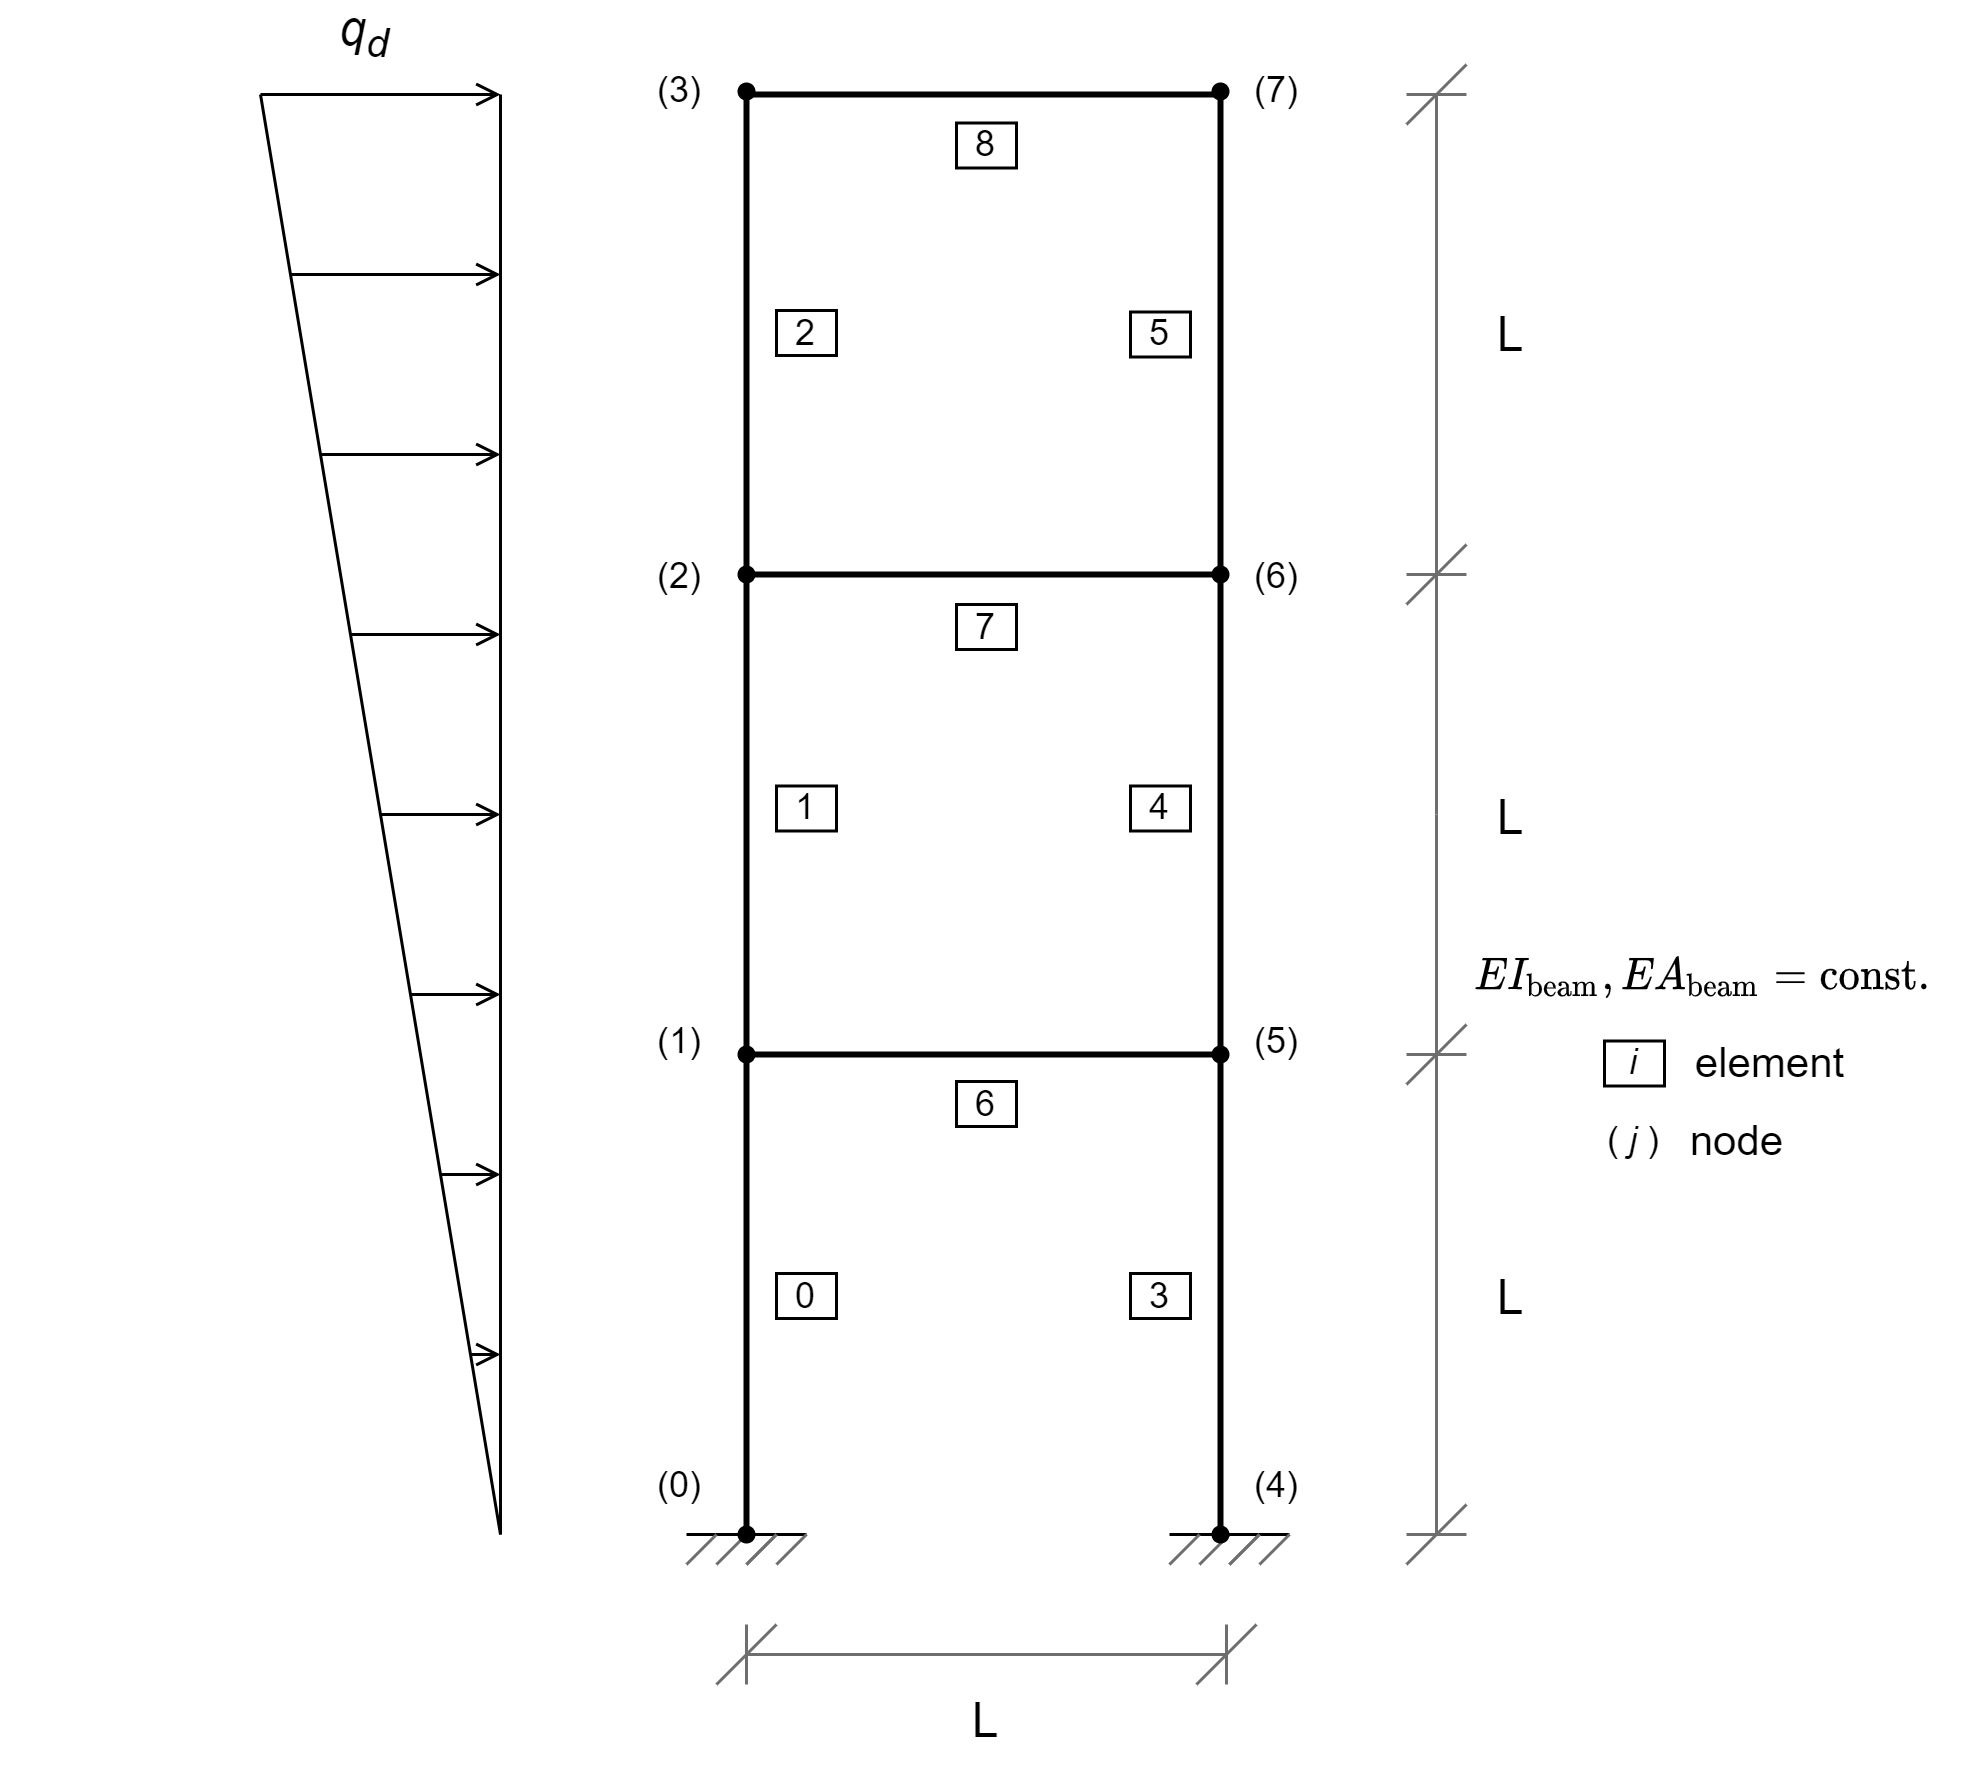
\includegraphics[width=\linewidth]{Figures/frameGeom.png}
	\caption{Structural system employed for the Case Study}
	\label{caseStudyGeom}
\end{figure}


The structure will be modelled using the \gls{FEM}, and more specifically, both for the beams and the columns, linear Euler-Bernoulli beam elements will be used. Three \glspl{DOF} will be accounted for at the elements' nodes, i.e. two translational (horizontal and vertical) and one rotational, all defined in the displayed 2D plane. At this point it should be noted that the elements of interest regarding their degradation, are the columns. This is a realistic simplification, bearing in mind that the deterioration and the possible failure of the columns can lead to more significant consequences and possibly to a global failure of the frame. Hence, as seen also in Figure \ref{caseStudyGeom}, both the axial and flexural stiffness of the beams are assumed to be constant. \\

In the same fashion as described in Section \ref{toyDescSec}, noisy measurements, e.g. accelerations obtained through a monitoring system, are passed through an output-only \gls{OMA} scheme, which yields modal data that are contaminated with additional noise, and are used as observations for the model updating procedure. In the current application, the first eigenmode is considered, meaning that a modal displacement will be observed for each of the eight ($8$) nodes, or to be more precise, for each of the six ($6$) nodes, since the two ($2$) bottom ones are fixed. This choice for the observed quantities serve for a better localization of the damage and the deterioration, which will eventually result in a more precise and beneficial maintenance strategy. For completeness reasons, the first three eigenmodes are illustrated in Figure \ref{eigModes}. 

\begin{figure}[H]
    \centering
    \begin{subfigure}[b]{0.33\textwidth}
        \centering
        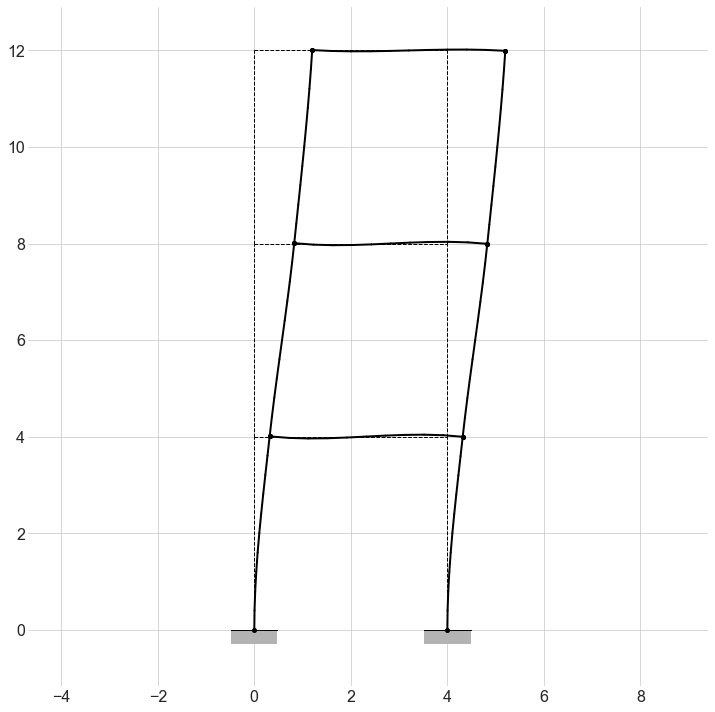
\includegraphics[width=\textwidth]{Figures/mode1.png}
        \caption{Mode 1}
        \label{m1}
    \end{subfigure}
    \begin{subfigure}[b]{0.33\textwidth}
        \centering
        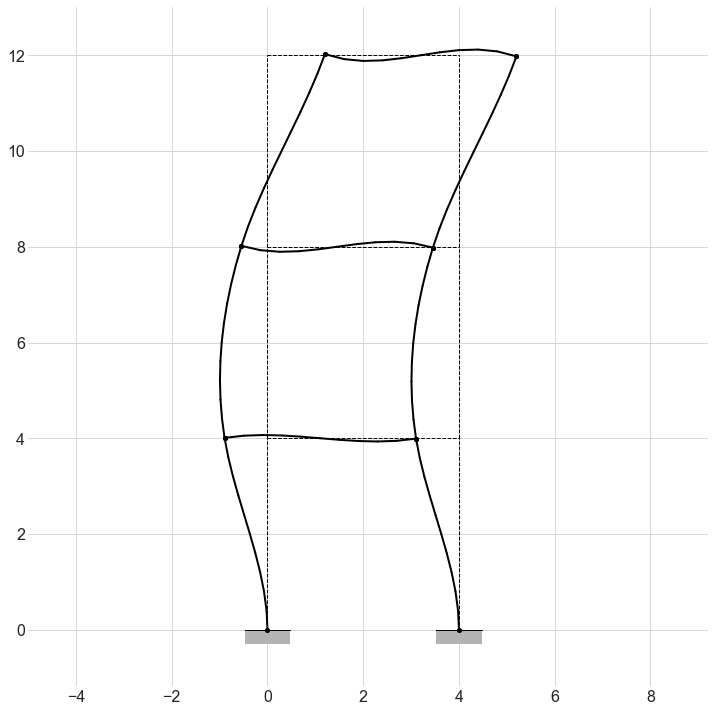
\includegraphics[width=\textwidth]{Figures/mode2.png}
        \caption{Mode 2}
        \label{m2}
    \end{subfigure}
    \begin{subfigure}[b]{0.33\textwidth}
        \centering
        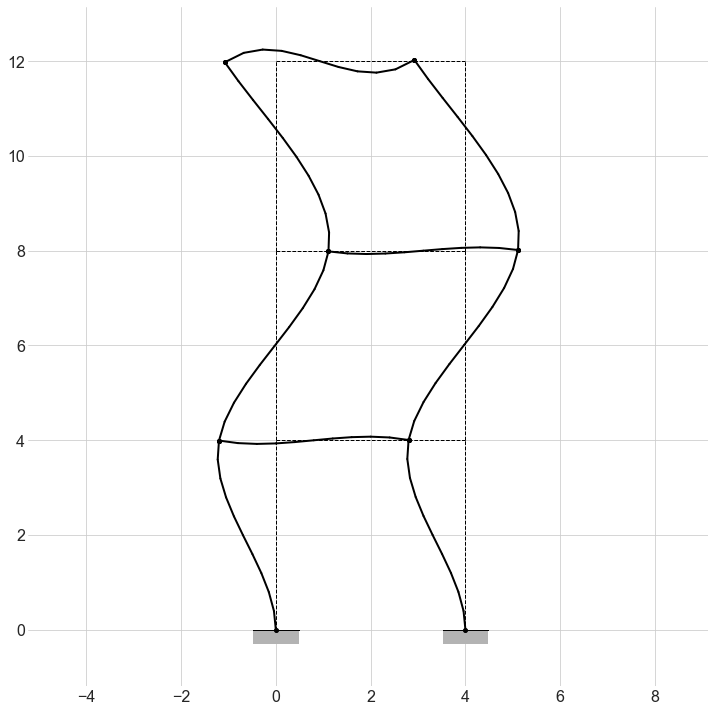
\includegraphics[width=\textwidth]{Figures/mode3.png}
        \caption{Mode 3}
        \label{m3}
    \end{subfigure}
    \caption{First three eigenmodes of the frame}
    \label{eigModes}
\end{figure}

It has already been mentioned that the reward, i.e. the maintenance cost, during each decision step, can be broken down into the cost of the taken action and the cost associated with the risk of failure (Equation \ref{rewardEq}). Therefore, in order to further elaborate on the concept of failure and quantify such a risk, and subsequently calculate the probability of failure, a \gls{SLS} check is employed. In particular, as stated in Clause 7.2.2 in EN 1993-1-1 \cite{EC3} and the Dutch National Annex to EN 1990, cl. A1.4.3(7), the limit of the horizontal displacement of the top storey, i.e. the drift, is $u\leq H/500$, where $H$ is the total height of the frame. Thus, for the structure at hand, failure has been reached if the drift of node (3) is greater than $H/500 = 12 \, \mathrm{m} / 500 = 0.024\, \mathrm{m} = 24\, \mathrm{mm}$. As far as the loading is concerned, a simple representation of seismic action is chosen. In particular, a triangular static equivalent load of maximum magnitude, $q_d$, is accounted for, which serves as an approximation of the first eigenmode of the structure. This assumption will reduce significantly the computational cost that would be induced by a dynamic time history analysis. The calculation of the triangular load's maximum value is included in Appendix \ref{annexLoad}. A more elaborate and realistic choice for the load (e.g. including the self weight of the transverse beams, etc) would not be beneficial for the scope of this project, since the assumed load case intervenes only in the calculation of the top storey drift and subsequently the probability and cost of failure. The \gls{DRL} and \gls{BMU} aspects of the problem are not affected by this modelling decision, which means that a simplified yet representative load will not affect the framework's accuracy.\\

The assumed material, cross-sections, dimensions and loads are summarized in Table \ref{problemDesc}.

\begin{table}[H]
    \centering
    \caption{Case study frame geometry and properties}
    \label{problemDesc}
    \begin{tabular}{cc}
        \toprule
        Beam cross section   & IPE220 \\
        Column cross section & HEA300 \\
        Material             & S355   \\ \midrule
        $L$                  & $4$ m    \\
        $q_d$                & $3.6$ kN/m    \\
        \bottomrule
    \end{tabular}
\end{table}

A simplified model in terms of discretization was chosen, i.e. one \gls{FE} per structural component, in view of reducing the computational cost. Owing to the relatively straightforward geometry, this decision does not cause any loss of accuracy, both for linear static and  eigen- analyses.

%------------------------------------------------------------------------------
%	ACTIONS
%------------------------------------------------------------------------------

\subsubsection{Actions}

In this multi-component application, a significant difference constitutes the fact that instead of a scalar action, there is an action \textit{vector} $\underline{a_t}$, containing at each decision step, the different actions that will be performed at the same time on every component. This can have a serious impact on the dimension of the global action-space, since for $n$ components and $m$ different action, there are $m^n$ possible action vectors in a combinatoric fashion. As a starting point, the same actions ($3$) presented in Section \ref{toyDescSec} and in Table \ref{actToy} are accounted for, which means that for the six ($6$) components of the frame, there are $3^6 = 729$ possible action vectors.\\

Similarly to the toy problem, the costs for the actions are expressed relatively to one another, as stated in Table \ref{costToy}, with the failure cost this time being significantly bigger. In particular, for the \gls{SDOF} oscillator, the failure cost was simply assumed twice as big compared to the replacement one, to account for the sudden nature of such an event and its consequences, but for the frame at hand, failure would mean a global collapse of the structure, so $C_{\text{F}} = 6 \, C_{\text{R}}$\footnote{six (6) is the number of the frame's components}. The extra cost that would be considered for this event happening abruptly is assumed to be compensated by the fact  that some of the relatively \textit{undamaged} components could possibly be reused. Therefore, the global failure would cost the same amount as a complete replacement of all the components. The relative values of the costs are included in Table \ref{costCase}. 

\begin{table}[H]
    \centering
    \caption{Rewards (costs) for the case study}
    \label{costCase}
    \begin{tabular}{lccc}
        \toprule
        \textbf{Description} & \textbf{Cost} & \textbf{Value} & \textbf{Factor} \\ \midrule
        Component's total replacement & $C_{\text{R}}$ & $C_0$ units & $1$ \\ 
        Component's partial repair & $C_{\text{M}}$ & $0.5\, C_{\text{R}}$ & $0.5$ \\
        Structure's global failure & $C_{\text{F}}$ & $6\, C_{\text{R}}$ & $6$ \\ 
        Risk of global failure & $C_{\text{risk}}$ & $P_f\,C_{\tet{F}}$ & $6\,P_f$ \\ \bottomrule
    \end{tabular}
\end{table}


%------------------------------------------------------------------------------
%	DETERIORATION MODEL/PROCESS
%------------------------------------------------------------------------------


\subsubsection{Deterioration Model}

As elaborated in Section \ref{detProcsSec}, a common and efficient approach regarding the modelling of the structure's degradation is the use of a Gamma process. The damage $d(\tau)$ is defined as the ratio of the current, degraded, cross section area over the initial one, i.e. $A(\tau)/A_0$. It is assumed that the corrosion penetrates the steel cross section uniformly (radially) meaning that all parts of the cross-section are equally exposed to the corrosive environment. Denoting the width of the degradation layer as $c$, Figure \ref{deterCrosSec} illustrates how the deterioration evolves on a cross-section scale.  

\begin{figure}[H]
    \centering
	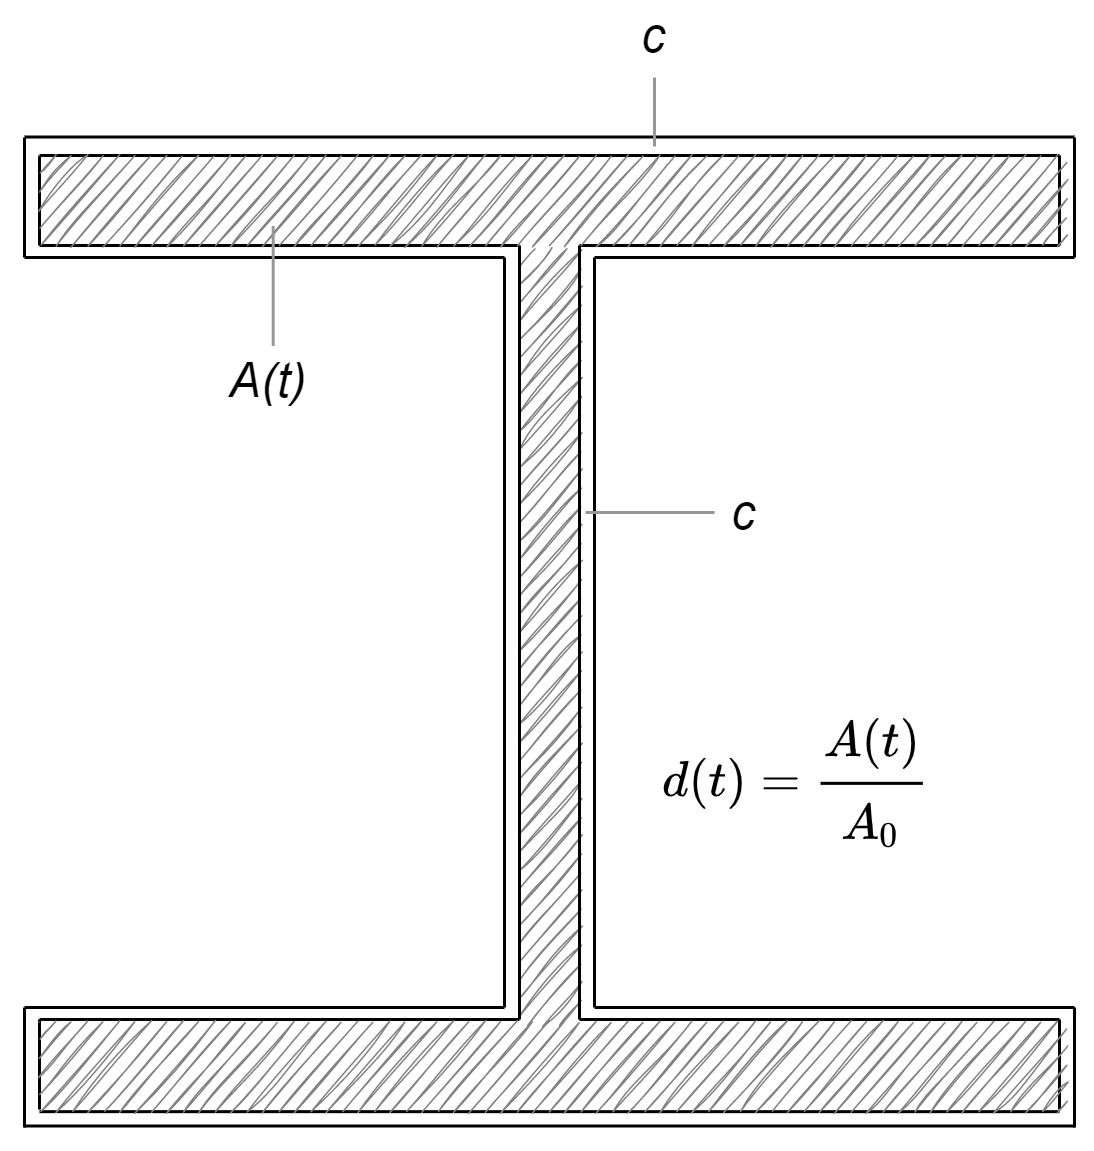
\includegraphics[width=0.4\linewidth]{Figures/crossSec.png}
	\caption{Degradation of the IPE cross-section}
	\label{deterCrosSec}
\end{figure}

Since the examined case is a 2D problem, the properties of interest, that intervene both in the linear static and the eigen- analysis, are the axial stiffness, $EA$, and the flexural stiffness, $EI$. With Young's modulus $E$ remaining constant, it is important to define the degradation of the moment of inertia, $I$, too. In Figure \ref{deterPlot} the deterioration of the cross section's properties is being plotted over the section loss percentage. The detailed calculations for the correlation between the two degradations (flexural and bending) are included in Appendix \ref{annexDeter}. 

\begin{figure}[H]
    \centering
	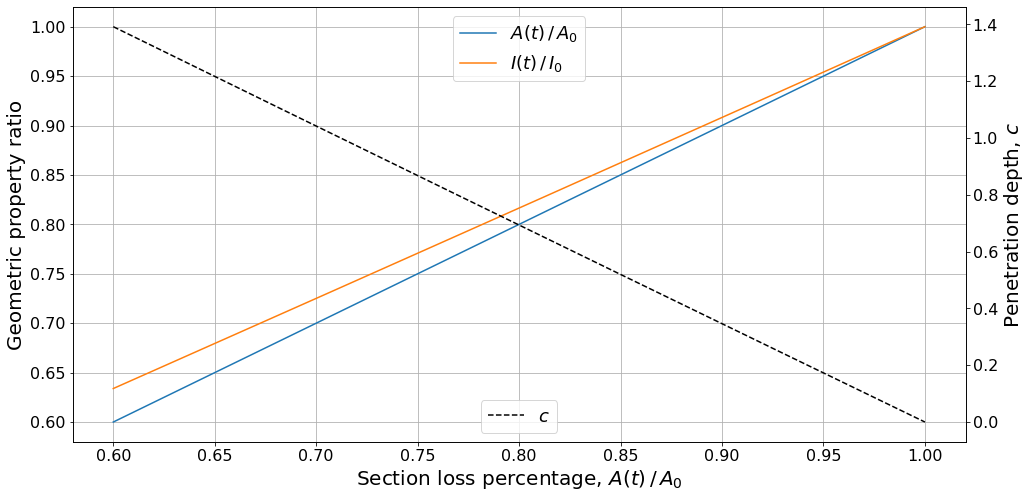
\includegraphics[width=0.85\linewidth]{Figures/deterPlot.png}
	\caption{Cross section properties deterioration}
	\label{deterPlot}
\end{figure}

Since the evolution of the deterioration follows a Gamma process, at every decision step the damage increment for each component is described by a Gamma distribution. Hence, as displayed also in Section \ref{detProcsSec}:

\begin{equation}
    \Delta D_i (\tau_i) \sim \mathrm{Ga}(v(\tau_i) - v(\tau_i - 1), u) \quad \text{for} \quad i = 1, \ldots 6 
\end{equation}

where $v(\tau_i)$ is the shape of the Gamma distribution for the deterioration rate of the $i$ component, and $u$ is the scale factor, assumed to be constant for all components.\\

In order to calculate the scale factor, $u$, it is assumed that the corrosive environment is affecting the structural components in such a way that after 70 years, there is a mean section loss of $40\%$ and a standard deviation 0f $7.5\%$, as chosen also in \cite{andriotis2019managing}. This means that:

\begin{equation}
    \left.
    \begin{array}{cc}
        \mathbb{E}\big ( d(70) \big ) = \cfrac{v(70)}{u} = 0.40  \\
        \mathrm{Var} \big ( d(70) \big ) = \cfrac{v(70)}{u^2} = 0.075
    \end{array}
    \right\}
    \Rightarrow u = 71.11
\end{equation}

Regarding the shape of the Gamma distributions though, a similar calculation is not possible, since $v(\tau)$ is the term where the stochasticity of the deterioration is accounted for. In particular, it is defined as follows:

\begin{equation}
    v(\tau) = A\,\tau ^B
\end{equation}

with $A, B$, being random variables. In a similar fashion with the toy problem, $A, B$ constitute the uncertain parameters which are initially assumed (prior knowledge) and are being updated using observations. Thus, during every decision step, a set of $A_i, B_i$ values is being sampled from the distributions $\prob{A}, \prob{B}$, for every component $i$, leading to a different Gamma distribution. Thus, the distribution of the total damage for each component at any given time/decision step is defined as the summation of all the Gamma distributions that describe the intermediate damage increments. It is known that the sum of gamma $(v_i, u)$ random variables has a gamma $(\sum v_i, u)$ distribution, thus:

\begin{equation}
    D_i^{\text{tot}} \sim \sum_{\tau = 1} ^T \mathrm{Ga} \big(\cdot \mid A^{\tau}_i \, \tau ^{B^{\tau}_i} - A^{\tau}_i \, (\tau - 1) ^{B^{\tau}_i}, u\big) = \mathrm{Ga} \big(\cdot \mid \sum_{\tau = 1} ^T A^{\tau}_i \, \tau ^{B^{\tau}_i} - A^{\tau}_i \, (\tau - 1) ^{B^{\tau}_i}, u\big)
\end{equation}

where $A^{\tau}_i, B^{\tau}_i$ are the values of $A, B$ sampled for a deterioration rate $\tau$ for the $i$ component\footnotemark.\\

\footnotetext{The Gamma distributions' shapes are dependent on the deterioration rate $\tau _i$ of each component, while the decision step counter, $t$, is global for the whole structure and it is evolving through unit increments until reaching the end of the episode, i.e. the time window of interest.}

The aforementioned details on the Gamma process, describe the so called \textit{transition step} for the updating of the belief, hence, the probability distribution for the deterioration of the structure. The other aspect of such an updating is the \textit{estimation step}, which is responsible for incorporating observations to improve the existing knowledge of the parameters of interest, i.e. $A, B$, with the use of a likelihood function. A graphical representation of the two, with the goal of defining the posterior distribution of the uncertain parameters is depicted in Figure \ref{beliefUpdFlow}.

\begin{figure}[H]
    \centering
	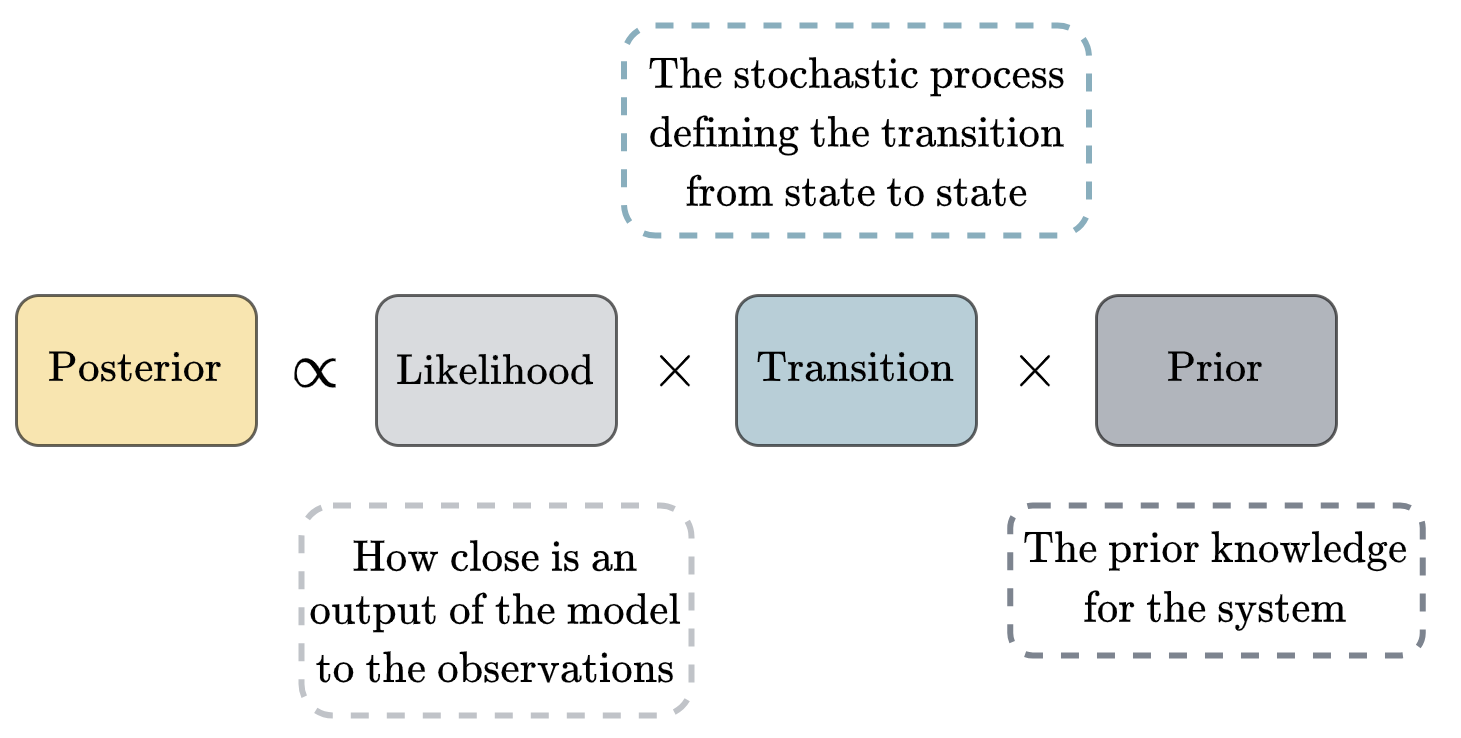
\includegraphics[width=0.7\linewidth]{Figures/beliefUpdate.png}
	\caption{Belief updating flowchart}
	\label{beliefUpdFlow}
\end{figure}

Denoting the system's parameters as $\theta = \langle A, B, \underline{D} \rangle$, and the observations, i.e. the modal displacements for the first eigenmode, as $\underline{O}$, the likelihood function is assumed to follow a normal distribution:


\begin{equation}
    \prob{\underline{O}\mid \underline{\theta}} = \Big (\prod _{k=1}^n \cfrac{1}{\sigma _k \, \sqrt{2\, \pi}}\Big) \cdot \exp{\Big[ -\sum _{k=1}^n \cfrac{\big(O_k - \mathrm{M}(\underline{\theta})\big)^2}{2\, \sigma_k^2} \Big]} \label{likeliEq}
\end{equation}

In Equation \ref{likeliEq}, $\mathrm{M}(\underline{\theta})$ represents the modal displacements for the first eigenmode that are derived from the \gls{FE} model, given the parameters $\theta$, while $\sigma_k$ is the standard deviation that describes the added noise from the \gls{OMA} scheme. For each noisy measurement (modal displacement) $m_k$ that is passed through the output-only \gls{OMA}, the observation that is used in the likelihood function is $O_k \sim \ccal{N}(m_k, \sigma_k)$, with $\sigma_k = m_k \cdot \text{Noise}$.\\

A schematic representation of the updating process for the deteriorating structure at hand is demonstrated in Figure \ref{caseBayes}.

\vspace{0.5cm}

\begin{figure}[H]
    \centering
    \makebox[\textwidth][c]{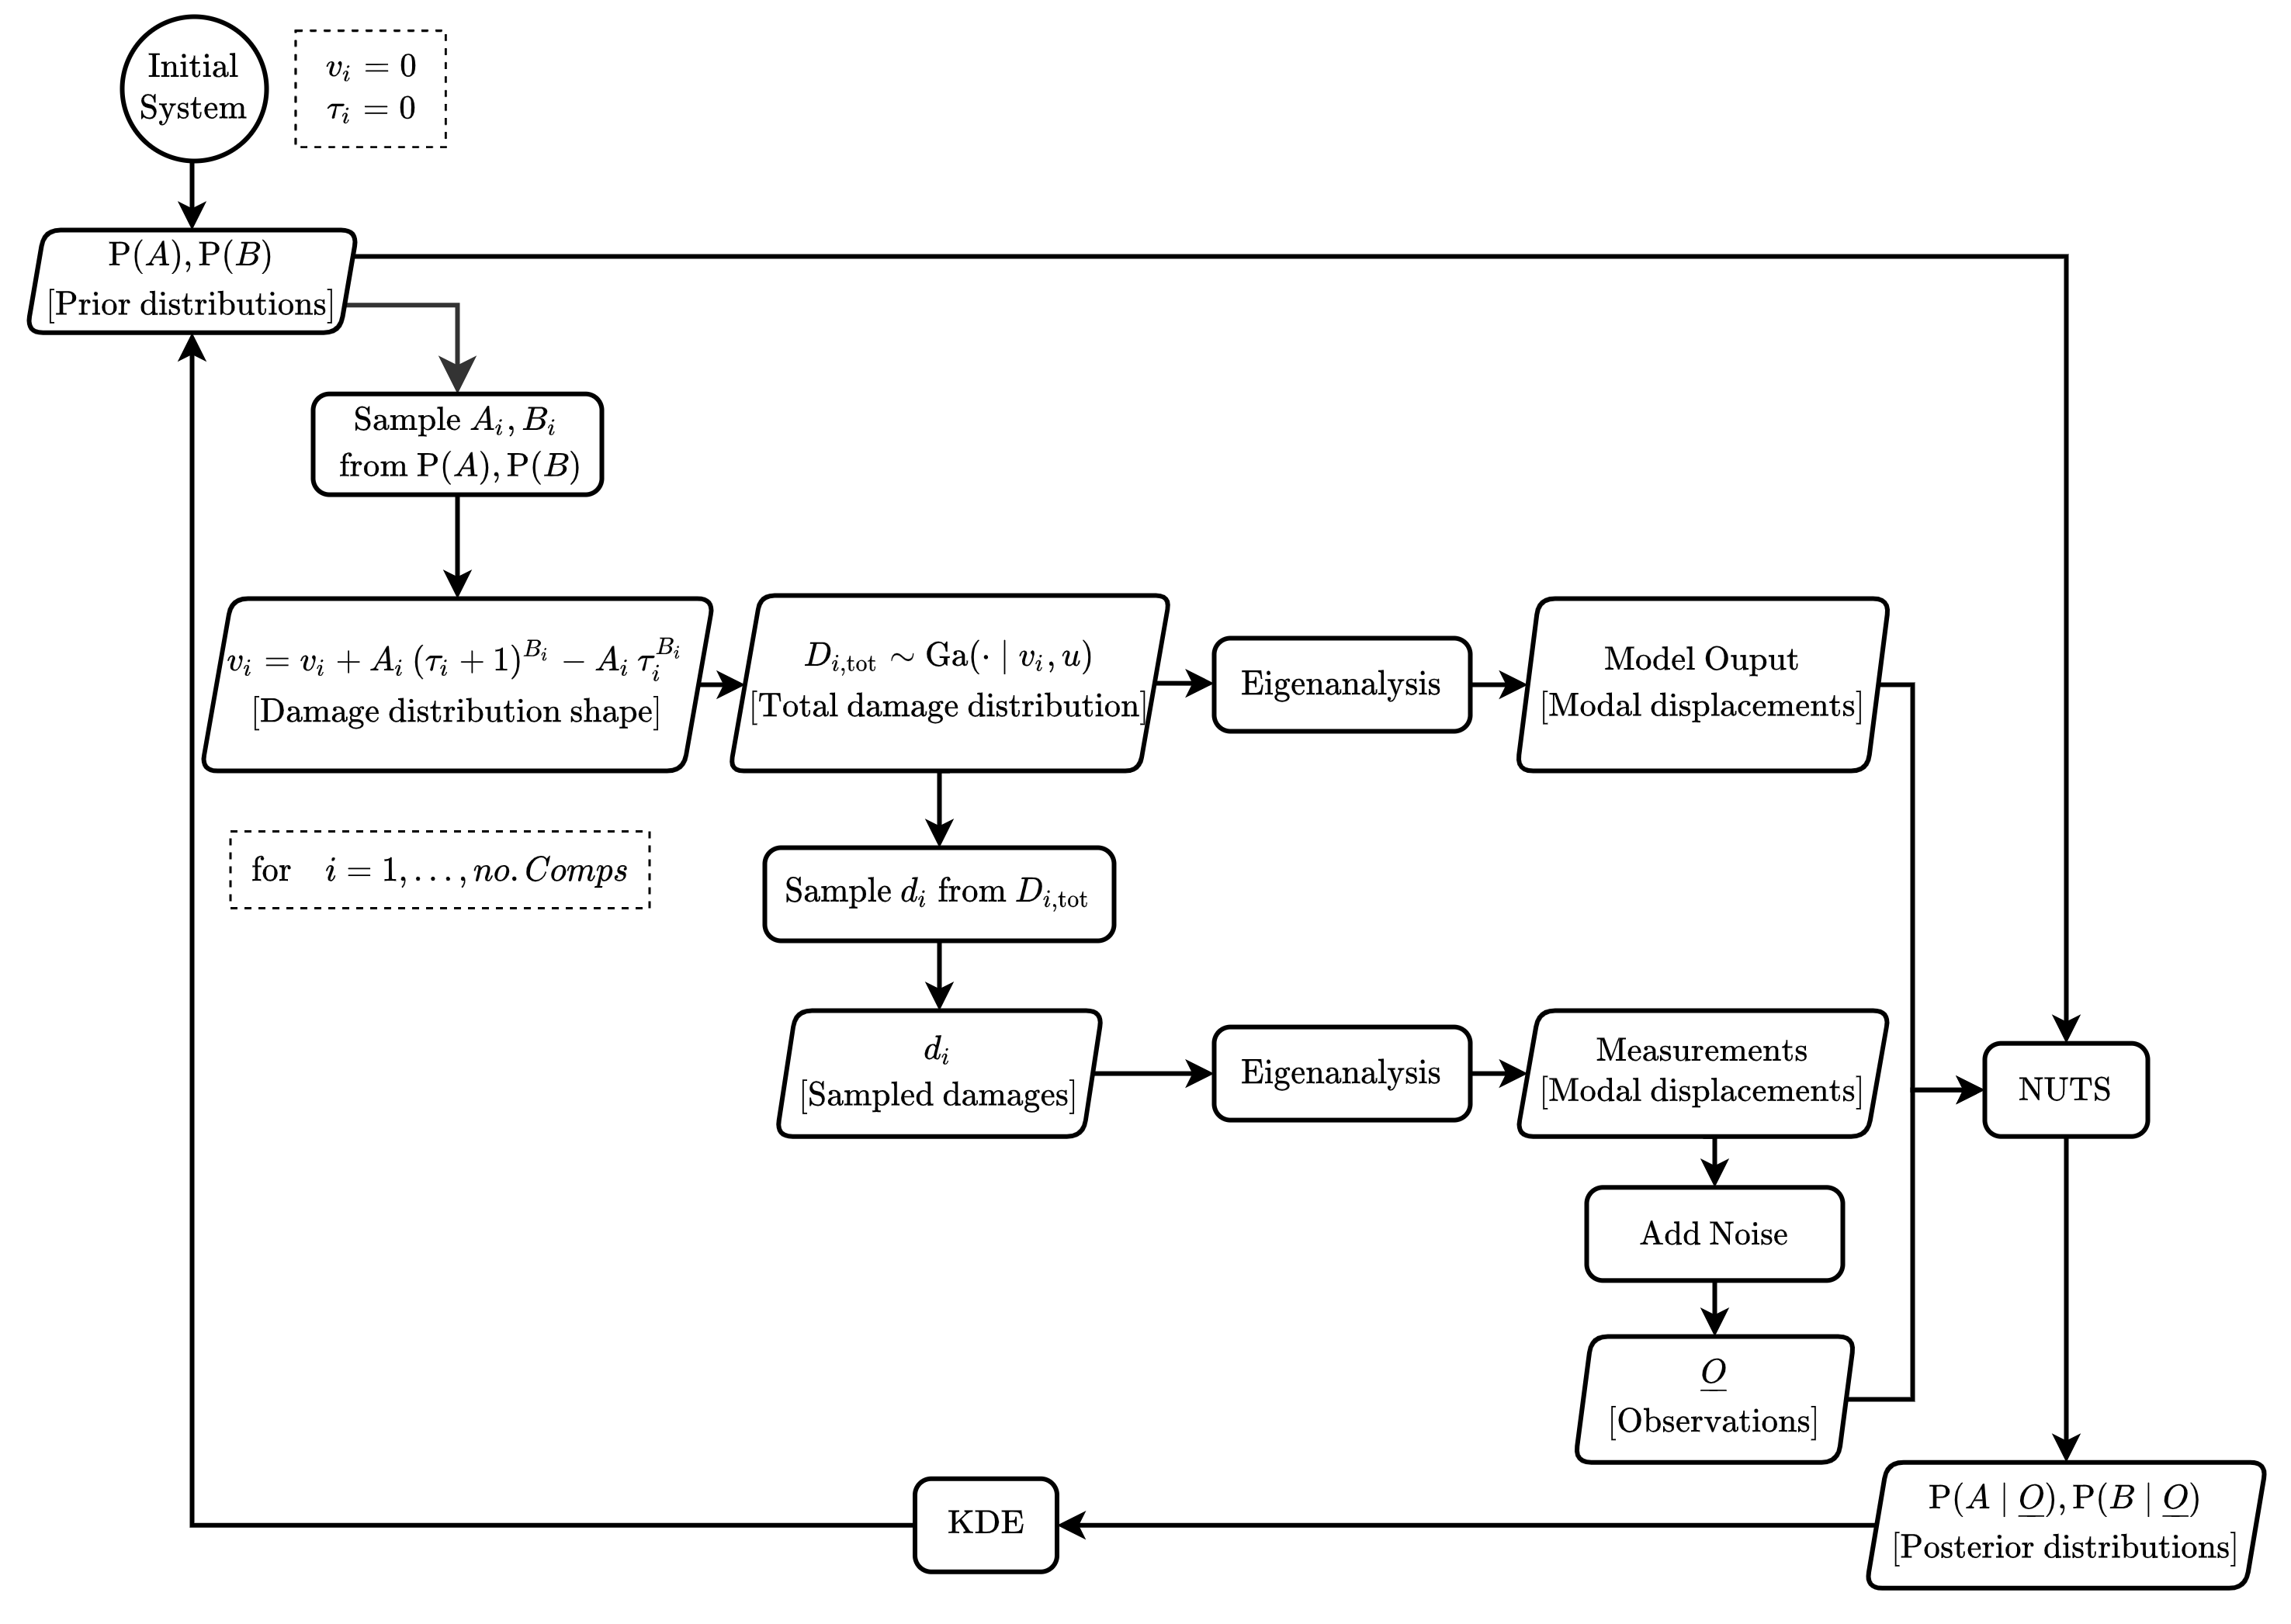
\includegraphics[width=1.1\textwidth]{Figures/caseBayesFlow.png}}
	\caption{Case Study Bayesian Inference}
	\label{caseBayes}
\end{figure}

\newpage
The same procedure is presented in a more technical and formal way in Algorithm \ref{bmuCase}.\\

\begin{algorithm}[H]
    \caption{Deterioration model parameters updating - Case Study}
    \algorithmfootnote{The dimensions of all the vectors are specified only at their first occurrence, i.e. $6x1$, and they always refer to the number of the structure's components}
    \label{bmuCase}
    \SetKwProg{Procedure}{DeteriorationParametersUpdating}{:}{}
    \SetKwProg{nuts}{\gls{NUTS}}{:}{}
    \SetKw{feEig}{\gls{FE}\_eigenanalysis}
    \Procedure{( $\prob{A}, \prob{B}$, \gls{FE} model, $u, T$ )}{
    Initialize $\mathrm{Ga(\cdot)}$ shapes $\underline{v}_{\,6x1} \gets \underline{\mathds{O}}_{\,6x1}$ \tcp{$\underline{\mathds{O}}$ is a vector of zeros} \\
    Initialize deterioration rates $\underline{\tau}_{\,6x1} \gets \underline{\mathds{O}}_{\,6x1}$\\
    
    \For {$t\gets 1$ \KwTo $T$}{
        Increment deterioration rates  $\underline{\tau} \gets \underline{\tau} + \underline{\mathds{I}}_{6x1}$ \tcp{$\underline{\mathds{I}}$ is a vector of ones}\\
        $\underline{A}_{\,6x1}, \underline{B}_{\,6x1} \gets$ sample from $\prob{A}, \prob{B}$ \\
        $\underline{v} \gets \underline{v} + \underline{A} \, (\underline{\tau} + 1)^{\underline{B}} - \underline{A}\,\,\underline{\tau} ^{\underline{B}}$\\
        Damage distribution of each component, $\underline{D}_{\,6x1} \sim \mathrm{Ga}(\cdot \mid \underline{v}, u)$\\
        $\underline{d}_{\,6x1} \gets$ sample from $\underline{D}$\\
        $\underline{\Delta u}_{\,0}_{\,6x1} \gets \feEig (\underline{d})$ \tcp{mean modal displacements, for the first eigenmode}\\
        
        Generate $\underline{\Delta u}_{\,\text{obs}}_{\,6x1} \gets \ccal{N}(\underline{\Delta u}_{\,0}, \text{ Noise})$\\ \vspace{0.2cm}
        \nuts{( $\prob{A}, \prob{B}, \underline{\Delta u}_{\,\text{obs}}$ )}{
        \KwOut{$\prob{A \mid \underline{\Delta u}_{\,\text{obs}}}, \prob{B \mid \underline{\Delta u}_{\,\text{obs}}}$}}\\
        Choose action, $\underline{a}_{\,t}_{\,6x1}$ \tcp{according to the \gls{PPO} agent}\\
        \For {$i \gets 1$ \KwTo $6$}{
            \If{$a_t^i$ is ``repair''}{
                $\tau_i \gets \mathrm{max}(0, \tau_i - 2)$ 
            }
            \ElseIf{$a_t^i$ is ``replace''}{
                $\tau_i \gets 0$\\
                $v_i \gets 0$
            }
        }
        $\prob{A}, \prob{B} \gets \prob{A \mid \underline{\Delta u}_{\,\text{obs}}}, \prob{B \mid \underline{\Delta u}_{\,\text{obs}}}$ \tcp{posteriors become priors through \gls{KDE}}
        }
    }
\end{algorithm}

\vspace{1cm}

\newpage

The (starting) values for the parameters of the model's deterioration are summarized in Table \ref{caseStudyInput}.

\begin{table}[H]
    \centering
    \caption{Case study input data}
    \label{caseStudyInput}
    \begin{tabular}{lccc}
        \toprule
        \textbf{Quantity} & \textbf{Value} & \textbf{Units} &  \\ \midrule
        Replace cost, $C_{\text{R}}$ & $10000$ & {[}-{]} &  \\
        Noise & $0.1$ & {[}-{]} &  \\
        Failure drift & $24$ & {[}mm{]} &  \\ \midrule
        \textbf{Parameter} & \textbf{Distribution} & \textbf{Mean} & \multicolumn{1}{c}{\textbf{\gls{CV}}} \\ \midrule
        $A$ & Lognormal & $0.1$ & \multicolumn{1}{c}{$0.5$} \\
        $B$ & Normal & $1.8$ & \multicolumn{1}{c}{$0.2$} \\ \bottomrule
    \end{tabular}
\end{table}


%------------------------------------------------------------------------------
%	PROBABILITY OF FAILURE
%------------------------------------------------------------------------------

\subsubsection{Probability of failure}

An important issue to be tackled is the calculation of the probability of failure, $P_f$, i.e. the drift of the top storey being $\geq 24\, \mathrm{mm}$, given the probability distributions of the components' damages. An \gls{MC} sampling would be the ideal solution in terms of accuracy, however it demands a significant amount of computational time. Thus, \gls{FORM} is chosen, and in particular, a geometric interpretation of it. To be more precise, as it has been thoroughly explained in \cite{cicirello2014efficient}, denoting $u_{\text{F}} = 24 \, \mathrm{mm}$ i.e. the failure drift, and $\mu(\underline{D})$ as the drift of the frame given the damage distributions of the components, $\underline{D}$, the \acrfull{LSS}\footnotemark is defined as:

\begin{equation}
    M(\underline{D}) = u_{\text{F}} - \mu (\underline{D}) = 0
\end{equation}

\footnotetext{In 2D problems, instead of a surface, there is the \gls{LSF}}

The \gls{LSS} separates the safe region, where $M(\underline{D}) > 0$, from the failure region, where $M(\underline{D}) < 0$, of the parameter space. The failure probability, $P_f$ can be expressed as the integral over the domain $M(\underline{D}) < 0$:

\begin{equation}
    P_f = \prob{M(\underline{D}) \leq 0} = \int _{M(\underline{D})\leq 0} \prob{\underline{D}} \mathrm{d}\underline{D} \label{pfIntegralEq}
\end{equation}

with $\prob{\underline{D}}$ being the joint \gls{PDF} for the uncertain components' damages $\underline{D}$.\\

A computationally inexpensive way to calculate the integral of Equation \ref{pfIntegralEq} is through a geometric optimization analysis. The two necessary steps to do so, are:

\begin{enumerate}
    \item Transform the uncertain variables, i.e. the damages, into independent normal basic variables $\underline{U}$ \footnotemark.
    \footnotetext{The most popular methods for this task are the Rosenblatt and the Nataf transformations}
    \item Compute the minimum distance $\beta$, the so-called \textit{reliability index}, of the \gls{LSS} from the origin of the standard coordinate system $\underline{U}$ as displayed in Figure \ref{FORMgeom}.
\end{enumerate}

The point closest to the origin, $U^*$, is referred to as the design point, and is the point with the highest joint density on the \gls{LSS}, meaning that it corresponds to the most probable combination of damages for the structure to fail.\\

The probability of failure can now be computed as:

\begin{equation}
    P_f = \int _{M(\underline{U})\leq 0} \prob{\underline{U}} \mathrm{d}\underline{U} \approx 1 - \Phi(\beta) = \Phi (-\beta)
\end{equation}

where $\Phi$ is the \gls{CDF} of a normally distributed random variable with zero mean and unit variance.

\begin{figure}[H]
    \centering
    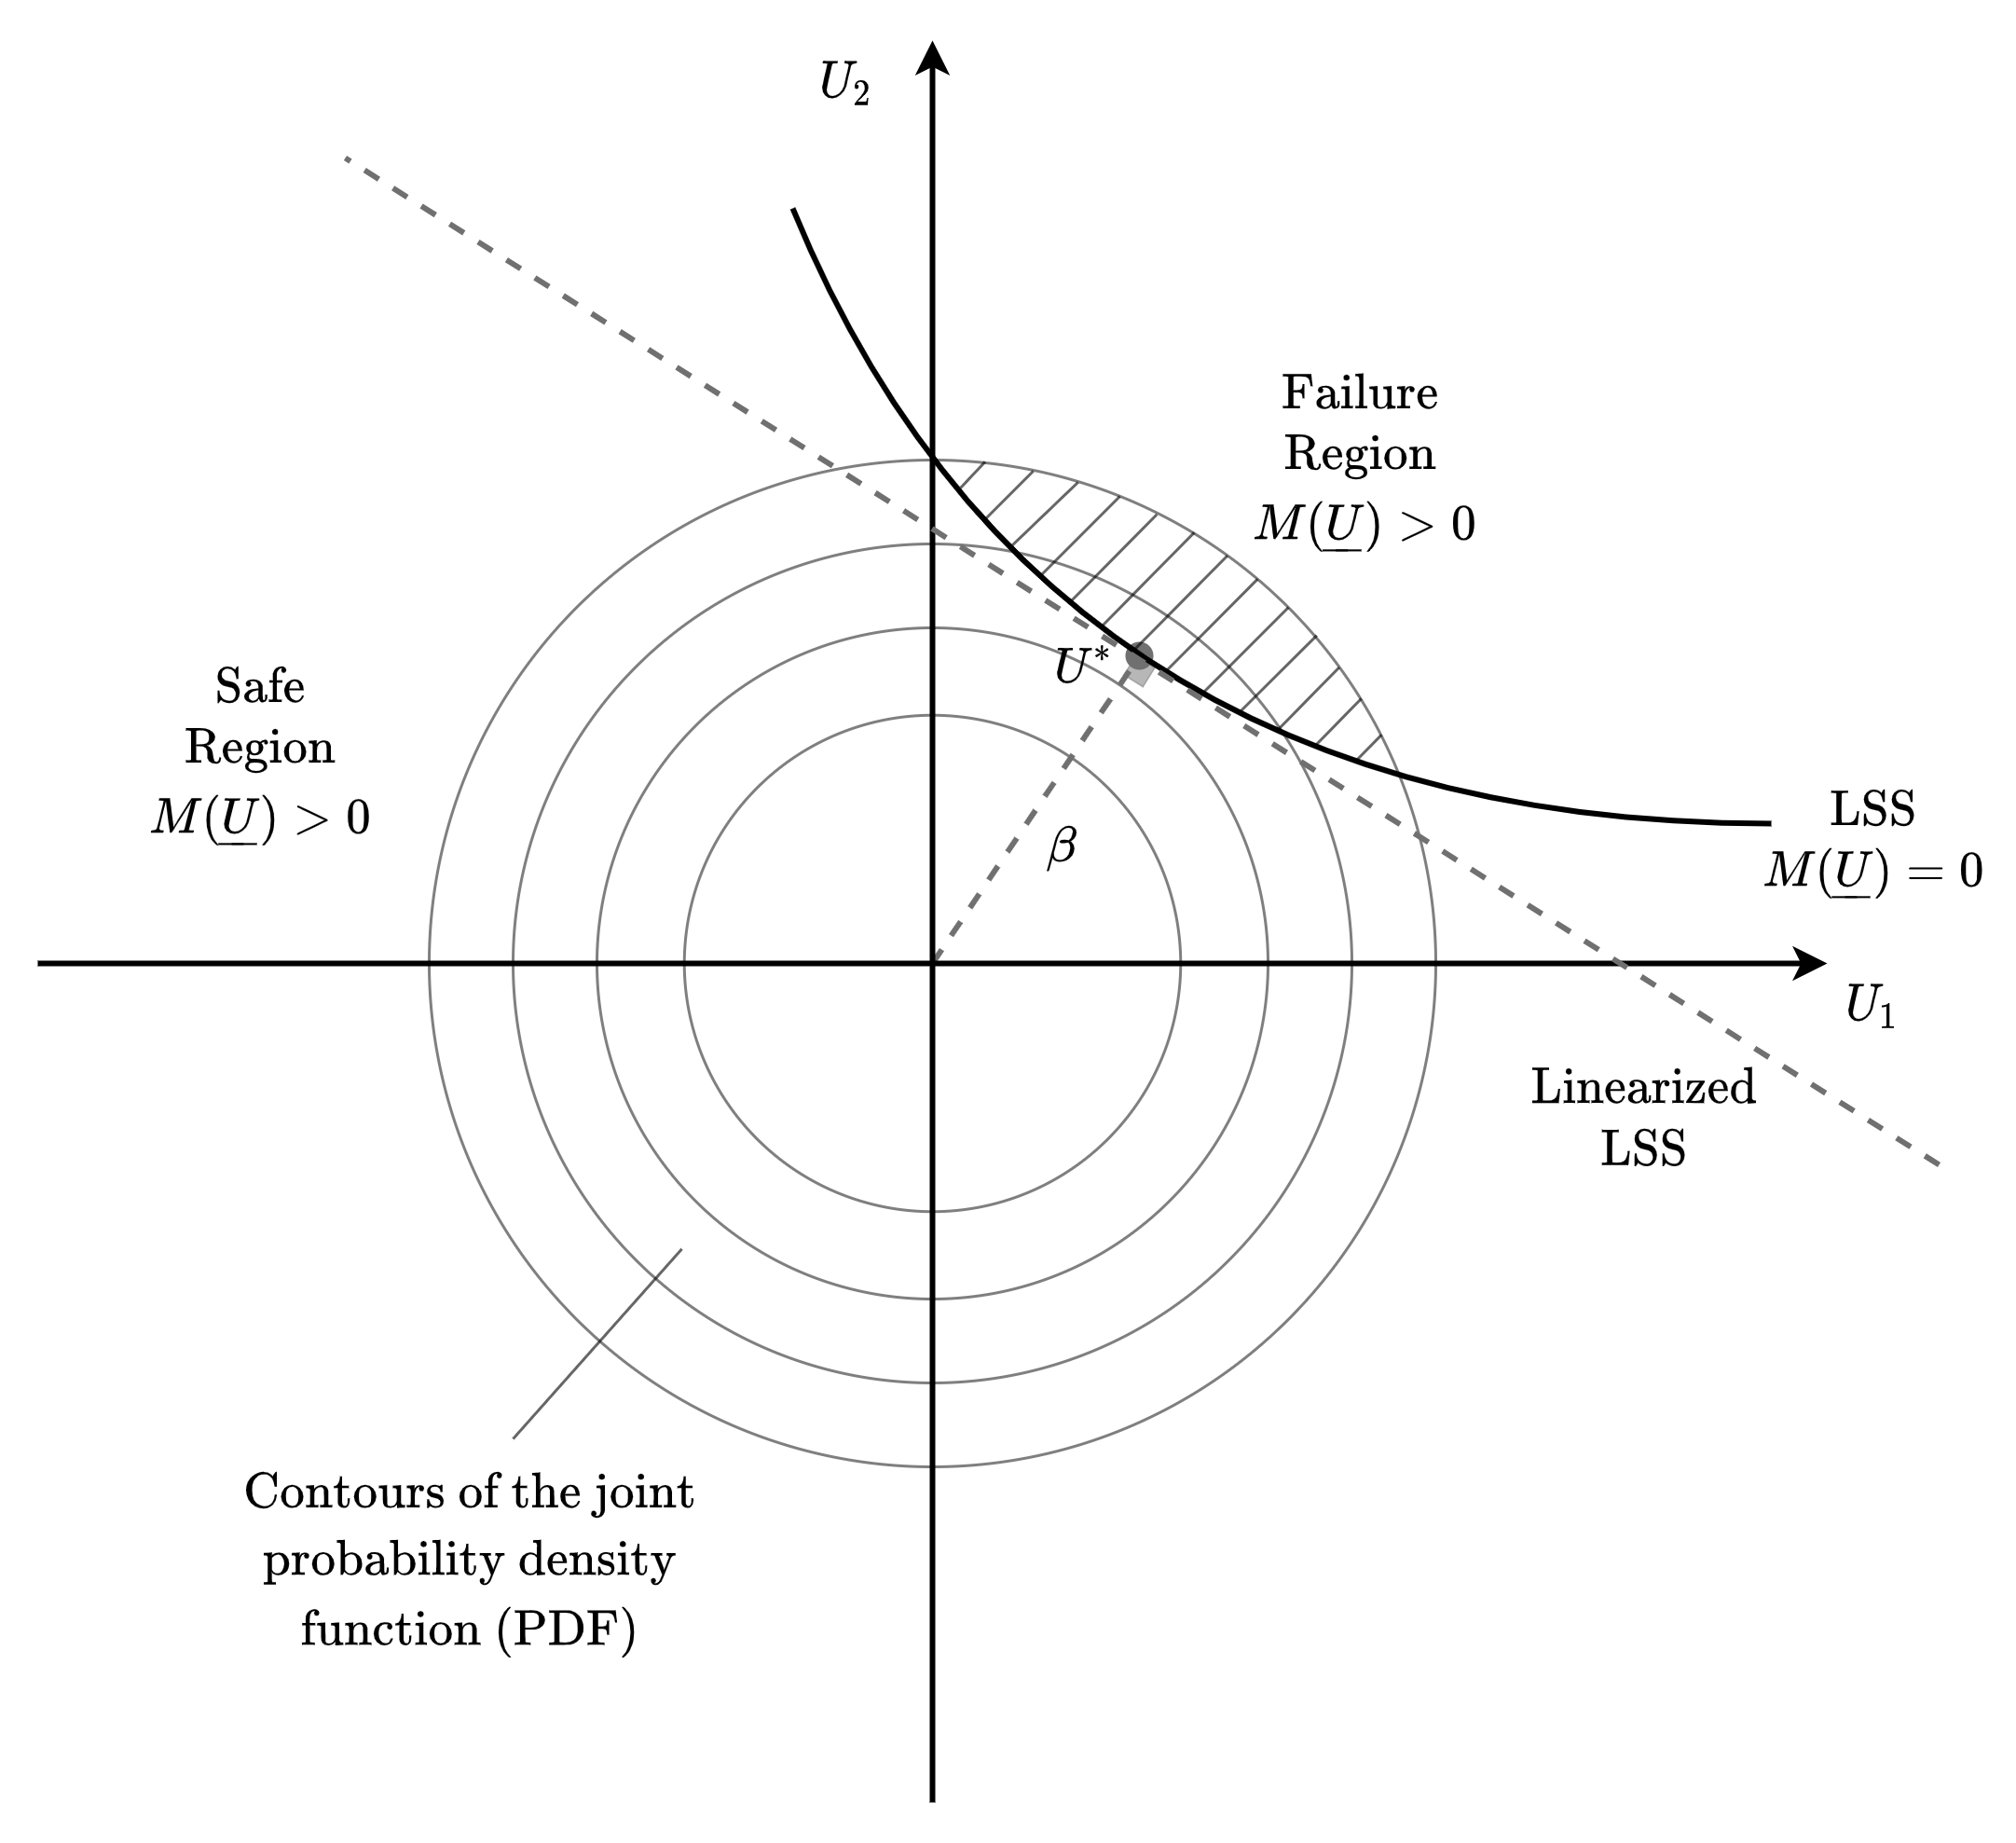
\includegraphics[width=0.8\textwidth]{Figures/FORM.png}
	\caption[Linearisation of the \gls{LSS} $M(\underline{U})=0$ at the design point $U^*$ in the uncorrelated standard normal random variables $\underline{U}$ space]{Linearisation of the \gls{LSS} $M(\underline{U})=0$ at the design point $U^*$ in the uncorrelated standard normal random variables $\underline{U}$ space \protect\footnotemark}
	\label{FORMgeom}
\end{figure}

\footnotetext{For clarity reasons, only two (2) standard normal variables are included in Figure \ref{FORMgeom}. For the case at hand, there will be a 6-dimensional space and subsequently, 6-dimensional hyperplane as an \gls{LSS}.}

\newpage

The step-by-step procedure followed to apply \gls{FORM} is exhibited in Algorithm \ref{formAlg}.\\

\begin{algorithm}[H]
    \caption{\acrfull{FORM} geometric interpretation}
    \algorithmfootnote{This procedure is not the exact function applied by the proposed framework, but the parameter updating in the absence of the \gls{DRL} aspect of the tool.}
    \label{formAlg}
    \SetKwProg{Procedure}{FORM}{:}{}
    \SetKw{feLinStat}{\gls{FE}\_linear\_static\_analysis}
    \Procedure{(Damage distributions $\underline{D}_{\,6x1}$, \gls{FE} model, failure threshold $u_F$ )}{
    Transform $\underline{D}$ into standard normal variables, $\underline{U}_{\,6x1}$\\
    $\mu (\underline{D}) \gets \feLinStat (\underline{D})$ \tcp{\gls{FE} model's drift}\\
    $M(\underline{D}) = u_F - \mu(\underline{D}) = 0$ \tcp{\acrfull{LSS}}\\
    Transform $M(\underline{D})$ to the normal space, $M(\underline{U})$\\
    $\beta \gets$ min distance between \gls{LSS} and the origin of $\underline{U}$ coord system \\
    $P_f \gets \Phi (-\beta)$
    }
\end{algorithm}

\vspace{0.5cm}

Even though \gls{FORM} is significantly lighter from a computational time point of view, it relies on the linearization of the \gls{LSS} to find the design point, $U^*$, which can lead to inaccuracies in highly non-linear problems. This is why, for the current application, which itself is not a linear problem, \gls{FORM}'s performance needs to be checked, through a comparison with a brute force \gls{MC} sampling approach. This comparison, as displayed in Figure \ref{formMcDiffs}, is made for three different amounts of samples, and for a 1000 different damage combinations and $P_f$'s.

\begin{figure}[H]
    \centering
    \begin{subfigure}[b]{0.48\textwidth}
        \centering
        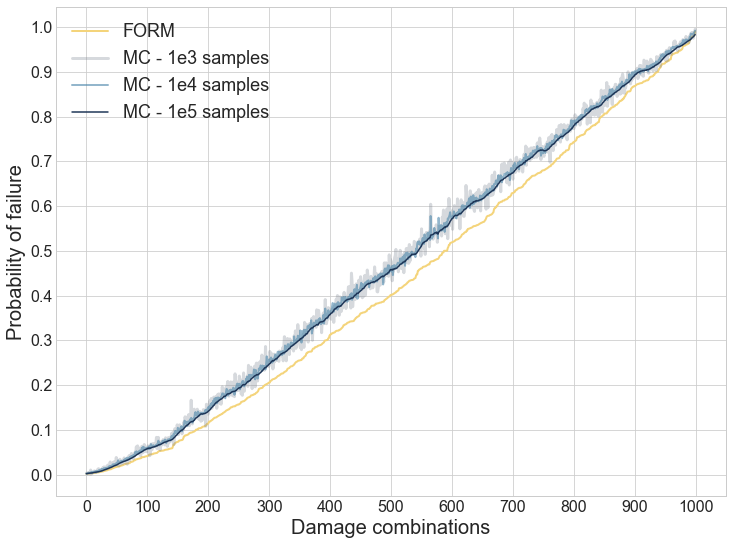
\includegraphics[width=\textwidth]{Figures/FORMvsMCpfs.png}
        \caption{$P_f$ for every approach}
        \label{formMcPfs}
    \end{subfigure}
    \begin{subfigure}[b]{0.48\textwidth}
        \centering
        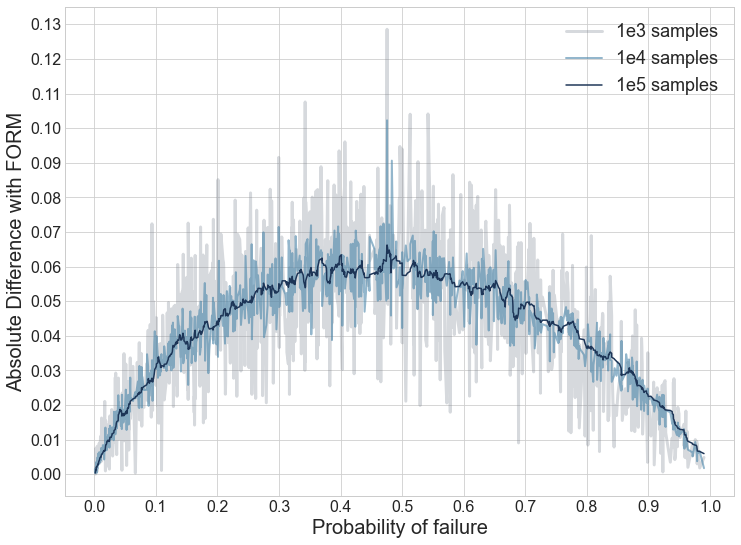
\includegraphics[width=\textwidth]{Figures/FORMvsMCabs.png}
        \caption{Absolute difference in $P_f$}
        \label{formMcAbsPf}
    \end{subfigure}
    \hfill
    \begin{subfigure}[b]{0.48\textwidth}
        \centering
        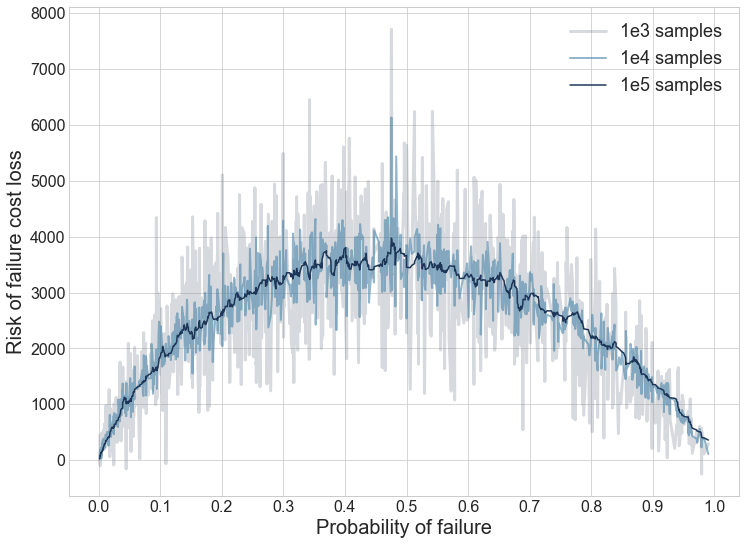
\includegraphics[width=\textwidth]{Figures/FORMvsMCriskFail.png}
        \caption{Absolute difference in $C_{\text{risk}}$}
        \label{formMcAbsRisk}
    \end{subfigure}
    \begin{subfigure}[b]{0.48\textwidth}
        \centering
        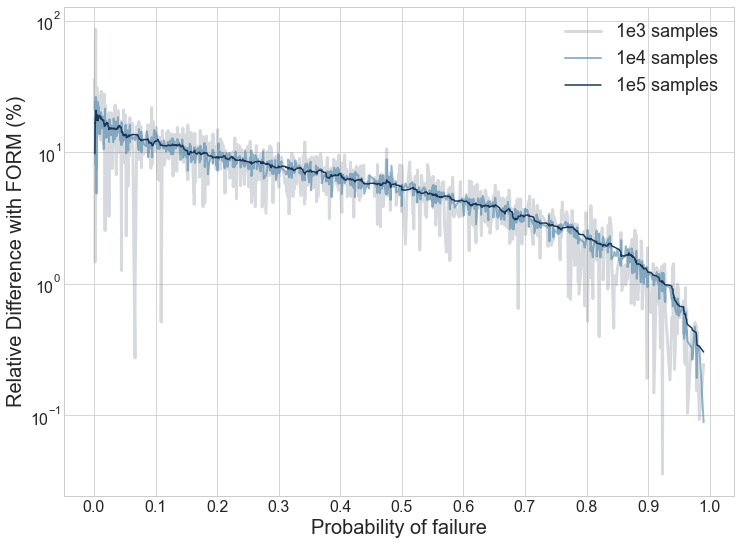
\includegraphics[width=\textwidth]{Figures/FORMvsMCrel.png}
        \caption{Relative difference (\%)}
        \label{formMcRelPf}
    \end{subfigure}
    \caption{Comparison between \gls{FORM} and \gls{MC}}
    \label{formMcDiffs}
\end{figure}

In Figure \ref{formMcPfs}, the probability of failure $P_f$ is plotted for different damage combinations, having applied all different approaches, meaning \gls{FORM} and \gls{MC} with 3 levels of samples. The results have been sorted and plotted in an ascending order of $P_f$ for a clearer representation. It can be observed that \gls{FORM} is consistently underestimating $P_f$, especially for values that are neither too big nor too small, i.e. approximately in the range of $0.1 - 0.9$. In the next two plots, i.e. Figures \ref{formMcAbsPf} and \ref{formMcAbsRisk}, it is highlighted that the absolute difference between the two approaches is not significant, especially again for either too small or too big values of $P_f$. What is more, it is again confirmed that higher values of $P_f$ are yielded with \gls{MC} sampling, which results also in higher risk of failure costs as seen in Figure \ref{formMcAbsRisk}. Lastly, the relative difference between the two methods, expressed as a percentage, is being plotted in logarithmic scale in Figure \ref{formMcRelPf}.\\

The accuracy of \gls{FORM} constitutes an important modelling aspect to be considered. Nevertheless, since it is capable of capturing small $P_f$'s and it will be employed both for the benchmark solution as well as the proposed framework, it is adequate for the time being, leaving some space for future improvements.




%------------------------------------------------------------------------------
%	FRAMEWORK
%------------------------------------------------------------------------------

\subsection{Framework} \label{caseFrameSec}


Regarding the \gls{DRL} aspect of the framework, not all of the algorithms examined in the current project are suitable for such an application. Owing to the multiple components, and the immense amount of possible action vectors, \gls{DDQN} would not perform efficiently for this case. As already been stated in the existing literature, \gls{DDQN} requires discrete action spaces, and the more the actions, the more difficult it is for the agent to arrive to optimal strategies. This is not the case with actor-critic algorithms, which based on the given state compute the probability distribution of the actions as an output, instead of the action-state value function. Thus, assuming that the actions of the the system's components are conditionally independent, the policy derived from an actor network, $\pi _{\theta}(\underline{a_t}\mid s_t)$, can be decomposed and expressed as the product of multiple policies which would refer to each component individually, $a_t^1, a_t^2, \ldots$ instead of the full action vector, $\underline{a_t}$. 

\begin{equation}
    \pi_{\theta}(\underline{a_t} \mid s_t) = \pi_{\theta}(a_t^1 \mid s_t) \cdot \pi_{\theta}(a_t^2 \mid s_t)\ldots \pi_{\theta}(a_t^6 \mid s_t) = \prod _{i=1}^6\pi_{\theta}(a_t^i \mid s_t)
\end{equation}

or,

\begin{equation}
    \log \big( \pi_{\theta}(\underline{a_t} \mid s_t) \big) = \sum _{i=1}^6 \log \big( \pi_{\theta}(a_t^i \mid s_t) \big)
\end{equation}



Therefore, the output layer of the actor network needs to have only $3 \times 6 = 18$ neurons, i.e. the probability of taking each action for each component. This means that every three output probabilities are summing up to one (1). A schematic representation of both the actor and the critic \glspl{DNN}, for \gls{PPO} \footnotemark is displayed in Figure \ref{casePPOnet}.\\

\footnotetext{Due to the poor performance of \gls{A2C} in both the discrete and continuous versions of the toy problem, it is not going to be tested for the case study, even though it could have handle the fact of multiple components, for it being an actor-critic algorithm.}


\begin{figure}[H]
    \centering
    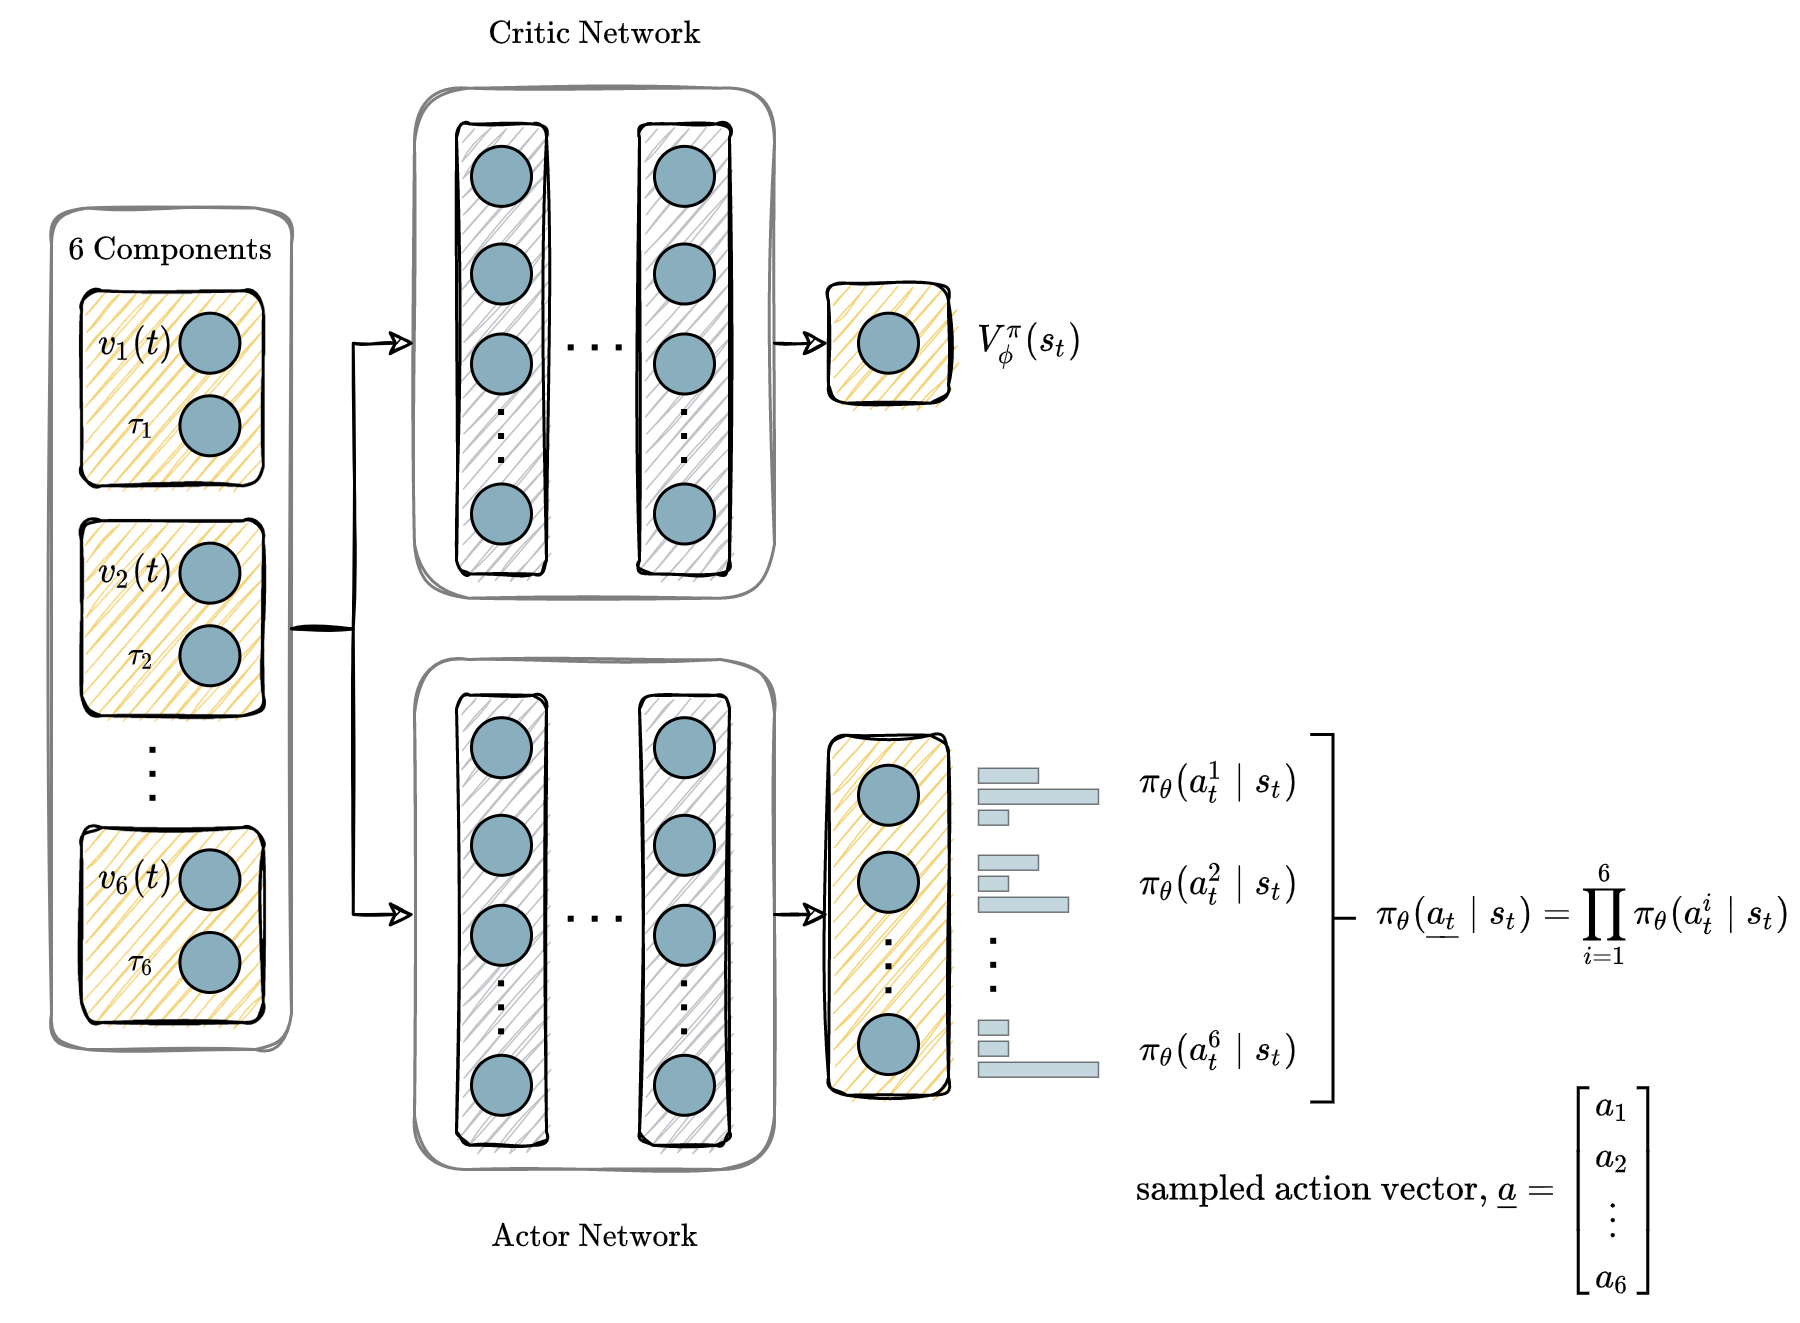
\includegraphics[width=\textwidth]{Figures/casePPOnet.png}
	\caption{\gls{PPO} architecture - Centralized states and actions}
	\label{casePPOnet}
\end{figure}

In the depicted architecture, instead of each component having its own agent, hence its own independent network, there is only one \textit{centralized} actor with shared parameters $\theta$ for all components. As elaborated also in \cite{andriotis2019managing} with \gls{DCMAC}, using such a network means that every agent is aware of all other agents' states, by getting as input the entire system state $s_t$, while being affected implicitly by their actions, too, through the common network weights $\theta$.\\

Various alternatives regarding the network architecture are presented as part of the future work in Section \ref{futDev}.

\loadgeometry{landscape}

Having elaborated on every aspect and sub-routine of the proposed framework, a summary of the complete procedure is illustrated in Figure \ref{flowCase}.

\vspace{1cm}

\begin{figure}[H]
    \centering
	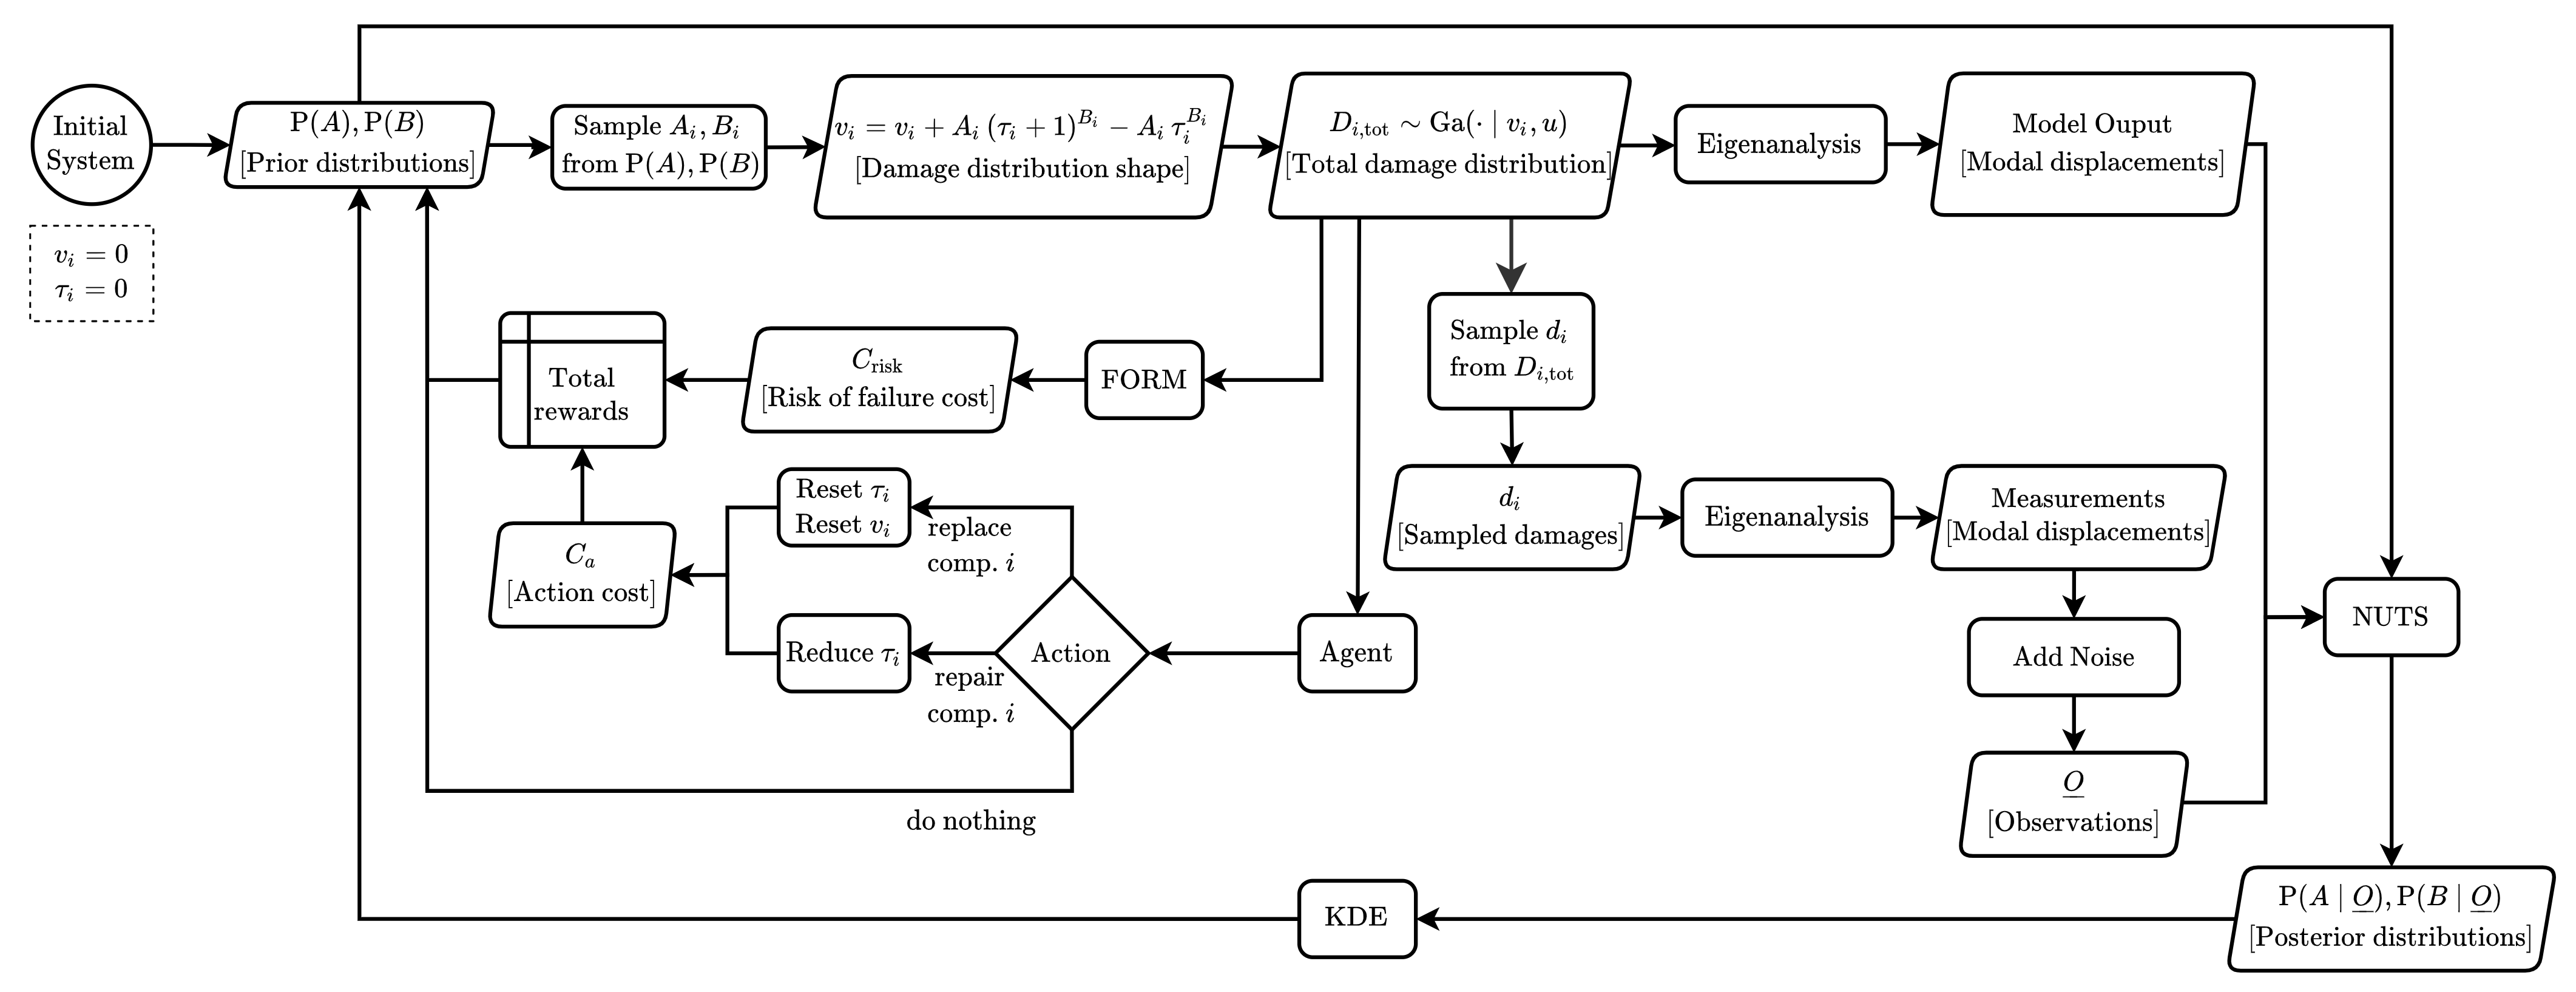
\includegraphics[width=\linewidth]{Figures/caseFlow.png}
	\caption{Case Study complete flowchart}
	\label{flowCase}
\end{figure}

\restoregeometry

Taking into account the \gls{DRL} aspect of the problem, and the steps included in the training of the \gls{PPO} agent, the developed tool is presented in a thorough and more formal way in Algorithm \ref{PPOcase}.\\

\begin{algorithm}[H]
    \caption{\acrfull{PPO} - Case Study}
    \algorithmfootnote{The indexing and slicing of vectors follows \texttt{Python} notation, i.e. $0$ is the starting index and the upper bound is exclusive.}
    \label{PPOcase}
    \SetKw{ppoTrain}{Train Agent}
    \SetKw{bmu}{\gls{BMU}}
    \SetKw{FORM}{\gls{FORM}}
    \SetKw{actor}{Actor Net}
    \SetKw{critic}{Critic Net}
    \SetKw{or}{or}
    Initialize policy (actor) network weights $\theta$\\
    Initialize value function (critic) network weights $\phi$\\
    \For {$episode = 1$ \KwTo $M$}{
        $s_t \gets$ reset environment \tcp{initialize $A, B$, $\underline{\tau}_{\,6x1} \gets \underline{\mathds{O}}_{\,6x1}$, $\underline{v}_{\,6x1} \gets \underline{\mathds{O}}_{\,6x1}$}\\
        \For {$t \gets 1$ \KwTo $T$}{
            $t \gets t + 1, \, \underline{\tau} \gets \underline{\tau} + \underline{\mathds{I}}$\\
            \bmu for params $A, B$ \tcp{procedure shown in Algorithm \ref{bmuCase}}\\ 
            $\pi _{\theta} (\underline{a}_t \mid s_t) \gets $ \actor ($s_t$) \tcp{$\pi _{\theta} (\underline{a}_t \mid s_t) = \pi _{\theta} (a_t^1 \mid s_t) \cdot \pi _{\theta} (a_t^2 \mid s_t) \ldots \pi _{\theta} (a_t^6 \mid s_t)$}\\
            $V_{\phi}(s_t) \gets $ \critic ($s_t$)\\
            $\underline{a}_t \gets$ sample from $\pi _{\theta} (\underline{a}_t \mid s_t)$ \tcp{$a_t^1$ from $\underline{a}_t[0:3]$, $a_t^2$ from $\underline{a}_t[3:6] \,\, \ldots$, $a_t^6$ from $\underline{a}_t[15:18]$}\\
            
            \For{$i \gets 1$ \KwTo $6$}{
                \If{$a_t^i$ is ``replace''}{
                    $\tau_i \gets 0$
                }
                \ElseIf{$a_t^i$ is ``repair''}{
                    $\tau_i \gets \text{max}(\tau_i - 2, 0)$
                }
            }
            $P_f \gets \FORM$ ($\underline{v}$) \tcp{the shapes of the Gamma (damage) distributions are passed as an input}\\
            $C_{a_t} \gets numReplaces \times C_{\text{R}} + numRepairs \times C_{\text{M}}$\\
            $R(s_t, \underline{a}_t) \gets C_{a_t} + P_f \, C_{\text{F}}$\\
            Observe next state $s_{t+1}$ \tcp{$s_{t+1} = \langle \text{shapes }\underline{v}, \text{ deterioration rates }\underline{\tau} \rangle$}\\ 
            Store tuple $\left( s_t, a_t, \pi _{\theta} (a_t \mid s_t), V_{\phi}(s_t), R(s_t,a_t) \right)$ in $\ccal{D}_k$ \tcp{$s_t = \langle \underline{v}, \underline{\tau} \rangle$}\\
            $s_t \gets s_{t+1}$\\
            \If{$t=T$ \or $n=N$}{
                \If{$t=T$}{
                    $V_{\phi} (s_{t+1}) \gets 0$\\
                    $s_t \gets$ reset environment \tcp{initialize $A, B$, $\underline{\tau} \gets \underline{\mathds{O}}$, $\underline{v} \gets \underline{\mathds{O}}$}
                }
                \Else{
                    $V_{\phi}(s_{t+1}) \gets \critic (s_t)$
                }
                Returns $\delta _t \gets R(s_t, \underline{a}_t) + \gamma \, V_{\phi}(s_{t+1}) - V_{\phi}(s_t)$\\
                Advantages $A_t \gets \delta _t + (\gamma \, \lambda ) \, \delta_{t+1} + \ldots + (\gamma \, \lambda ) ^{T-t+1} \delta _{T-1}$\\
                Store $\delta _t, A_t$ in $\ccal{D}_k$\\
                
            }
        }
        \ppoTrain($\ccal{D}_k$)
    }
\end{algorithm}

\newpage

The steps needed to train the \gls{PPO} agent for the case study, i.e. the function ``\textit{Train Agent}'' are demonstrated in Algorithm \ref{PPOtrainAgentCase}.\\

\begin{algorithm}
    \caption{\acrfull{PPO} agent training - Case study}
    \label{PPOtrainAgentCase}
    \SetKwProg{ppoTrain}{Train Agent}{:}{}
    \ppoTrain{($\ccal{D}_k$)}{
            Update parameters $\phi$, using the Critic cost function:
            $$L^{\text{VF}}(\phi) = \sum_{t=1}^{T} \left ( V_{\phi}(s_t)-\delta_t \right ) ^2 $$\\
            Update parameters $\theta$, using the Actor loss function:
            $$L^{\text{CLIP}}(\theta) = \sum_{t=1}^{T} \min \left(\cfrac{\pi_{\theta}\left(\underline{a}_t \mid s_{t}\right)}{\pi_{\theta_{\text{old}}}\left(\underline{a}_t \mid s_{t}\right)} A_t \left(s_{t}, \underline{a}_{t}\right), \, \text{clip} \left( \cfrac{\pi_{\theta} \left( \underline{a}_t \mid s_{t} \right )}{\pi_{\theta_{\text{old}}} \left( \underline{a}_t \mid s_{t} \right )}, 1-\varepsilon, 1+\varepsilon \right) A_t \right)$$
            via minibatch stochastic gradient ascent with Adam
        }
        
\end{algorithm}

\newpage

%------------------------------------------------------------------------------
%	BENCHMARKING
%------------------------------------------------------------------------------

\subsection{Benchmarking}

For the sake of comparison and evaluation of the proposed framework, a benchmark approach needs to be applied on the case study, setting the threshold (in terms of cost) that the \gls{PPO} agent will try to surpass.\\

As mentioned also for the toy problem in Section \ref{toyBenchSec}, usually a heuristic approach is chosen, which indicates when it is more beneficial to perform a maintenance action based on a variety of metrics. Common options are the maximum damage allowed (per component), the maximum probability of failure of the structure as a whole, or even a time threshold which would specify every how many decision steps (e.g. years) a maintenance action should be performed.\\

Although, for the \gls{SDOF} system, the control quantity would not lead to considerable differences, it is expected, that for a multi-component system, monitoring the deterioration of each component separately can lead in a more efficient maintenance strategy and life-cycle cost. Nevertheless, both the optimal damage threshold and the optimal maintenance time interval will be sought, and ultimately the yielded results of these two heuristic approaches, namely \gls{CBM} benchmark and \gls{TBM} benchmark, will be compared with the ones of the proposed methodology.\\

Regarding the \gls{CBM} benchmark, a fine grid of repair and replace thresholds is created, in order to check which combination would yield the minimum maintenance cost. In particular, increments of $0.05$ are considered starting from $0$ damage, up to $0.5$. Due to the high stochasticity of the corrosive environment, an abundance of episodes was ran for each pair of values. The obtained thresholds as well as the resulting maintenance cost mean and standard deviation are displayed in Table \ref{benchValuesCase}, while a policy realization of such a heuristic approach is depicted in Figure \ref{benchCasePol}.

\begin{table}[H]
    \centering
    \caption{\acrshort{CBM} Benchmark maintenance thresholds and costs - Case Study}
    \label{benchValuesCase}
    \begin{tabular}{cccc}
        \multicolumn{2}{c}{\textbf{Optimal Thresholds}} & & \\ \toprule
        \textbf{Repair} & \textbf{Replace} & \textbf{Mean Cost} & \multicolumn{1}{c}{\textbf{St. Dev.}} \\ \midrule
        None & $0.10$ & $\boldsymbol{117819.96}$  & $25854.85$ \\ \bottomrule
    \end{tabular}
\end{table}

As displayed also in Table \ref{benchValuesCase}, according to the benchmark, it is more beneficial to let the components deteriorate and perform directly a replace action when $0.10$ damage is reached, rather than perform a partial repair earlier.

\newpage

A realization of a maintenance policy following the benchmark approach, i.e. heuristic damage thresholds, is displayed in Figure \ref{benchCasePol}.

\begin{figure}[H]
    \centering
    \makebox[\textwidth][c]{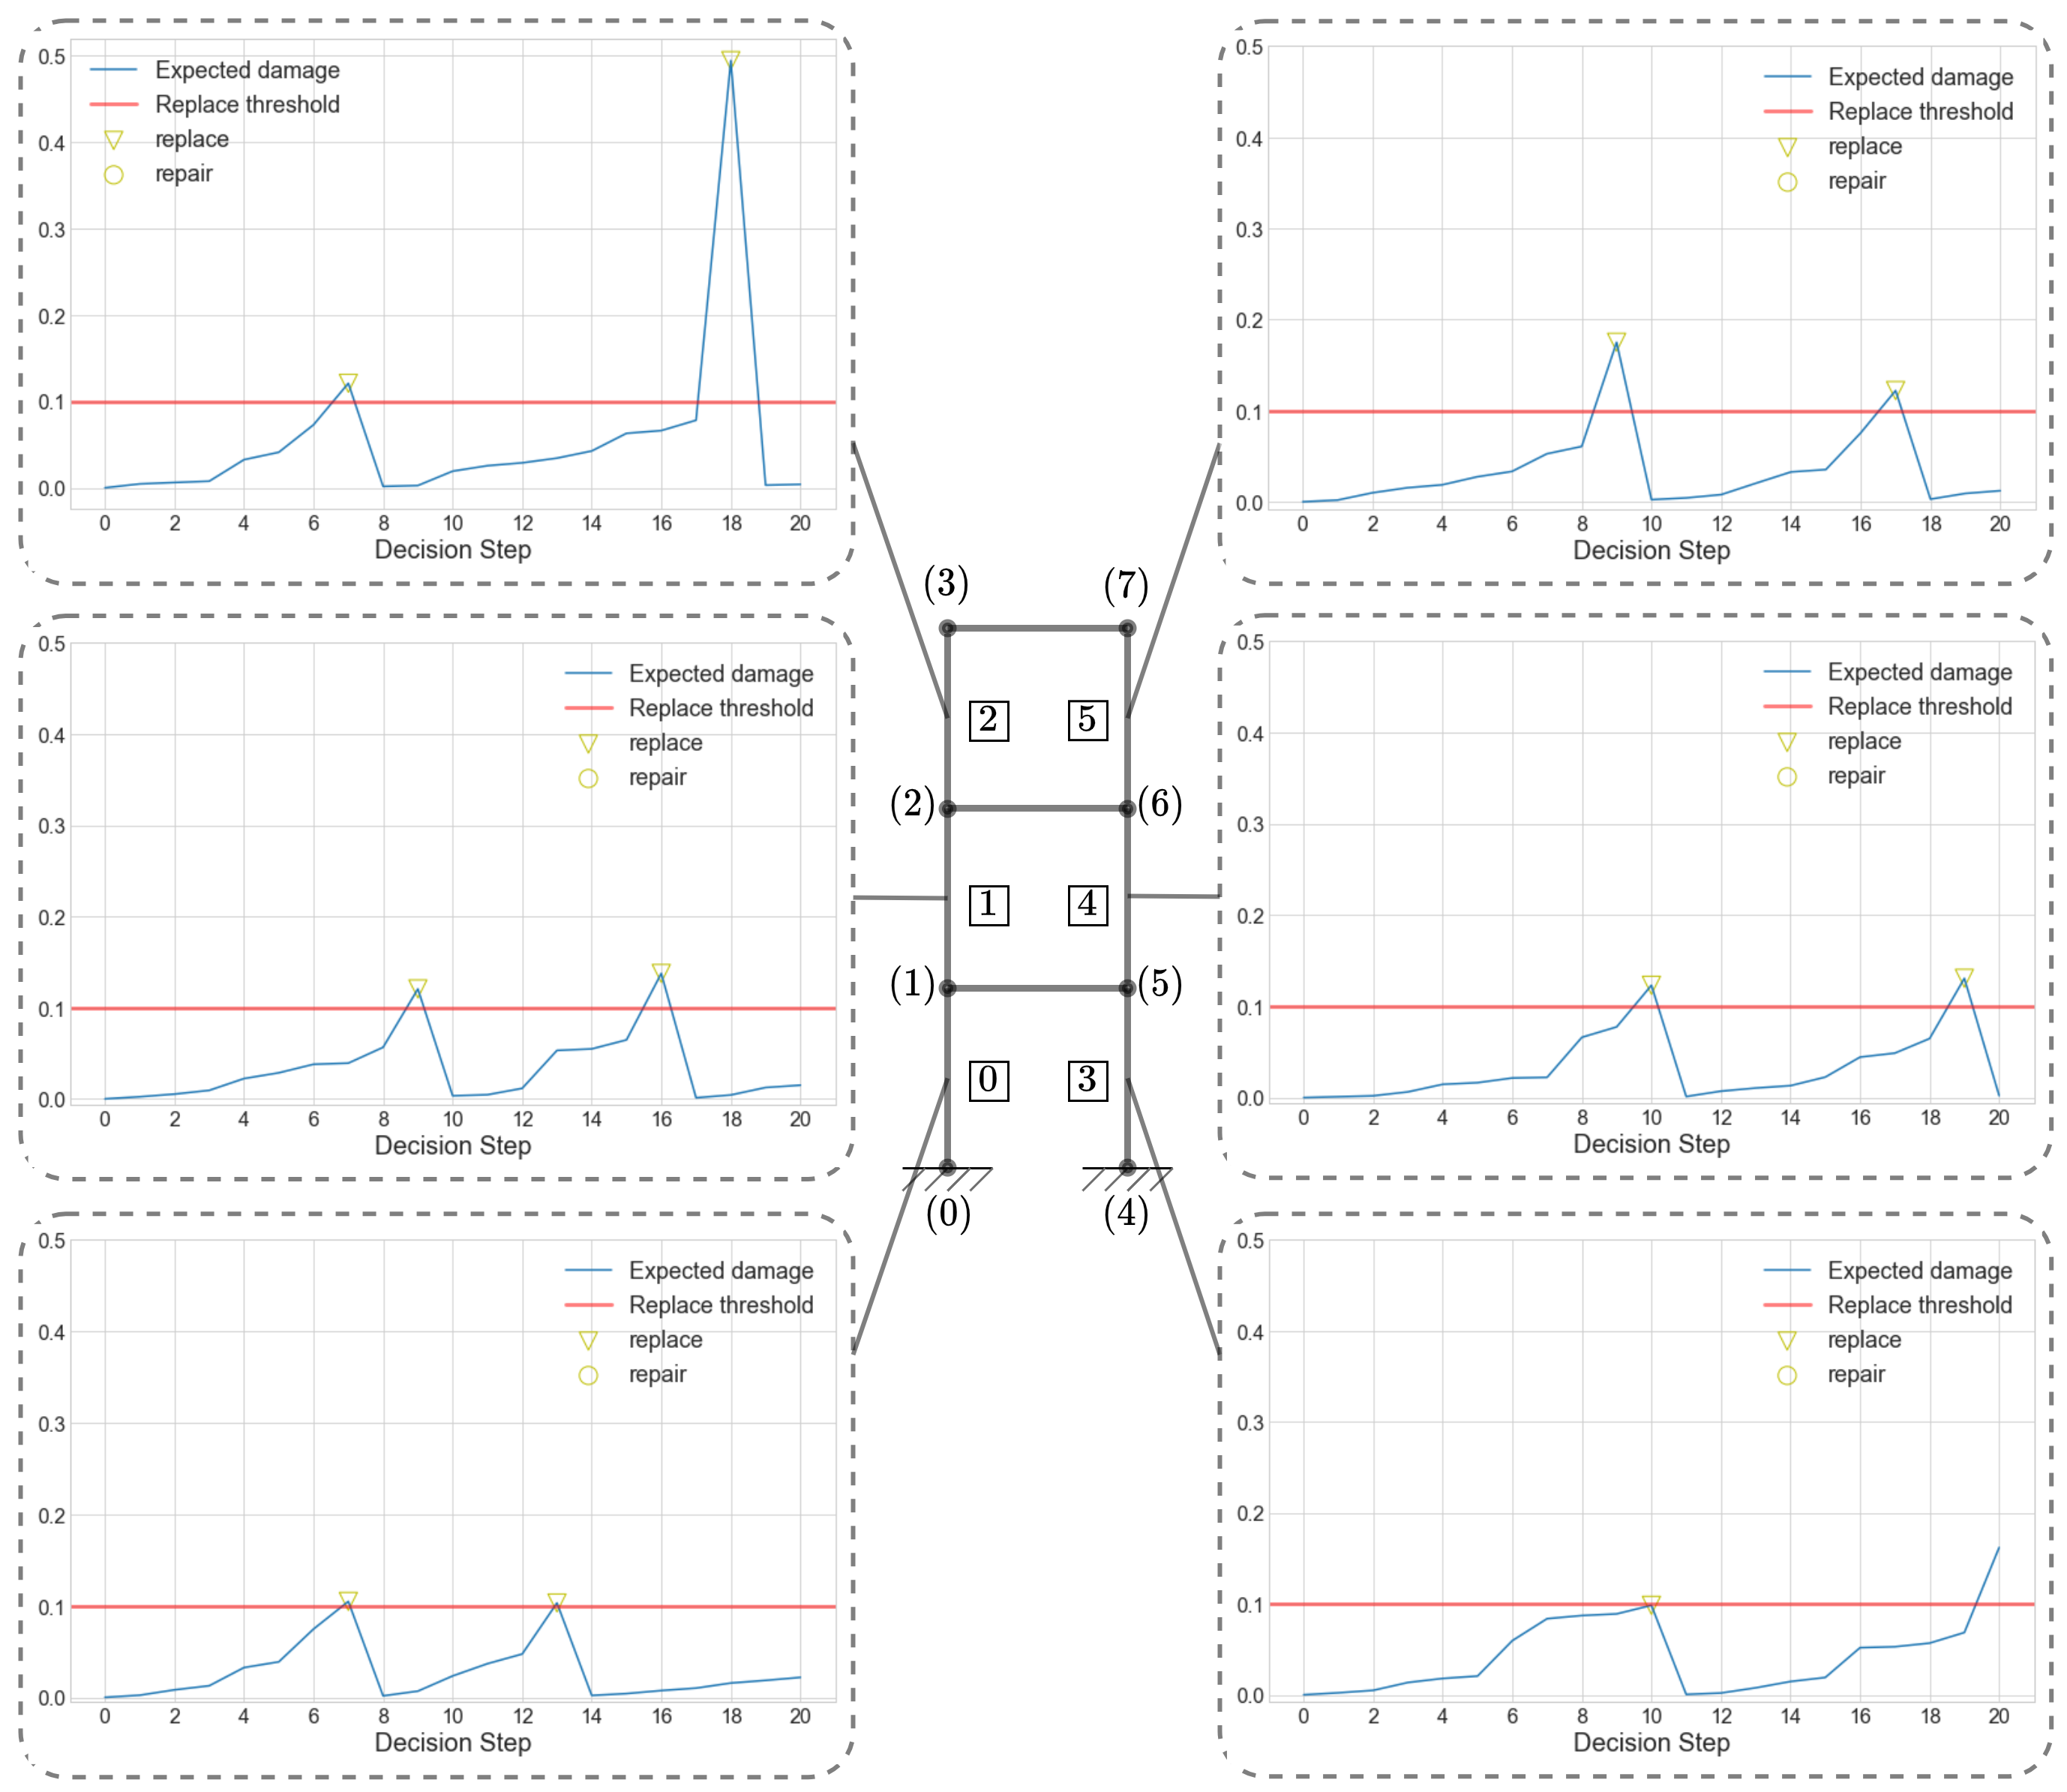
\includegraphics[width=1.2\textwidth]{Figures/benchCasePol.png}}
	\caption{Policy realization for all components - \acrshort{CBM} Benchmark}
	\label{benchCasePol}
\end{figure}

\newpage

As far as the \gls{TBM} benchmark is concerned, once more a plethora of threshold combination was examined, as well as a great amount of episodes due to the stochastic nature of the environment. The scenario of performing replace actions to all components periodically was considerably more beneficial compared to partial repairs. The different maintenance costs obtained for the different replace intervals are plotted in Figure \ref{tbmRplIntervals}. 

\begin{figure}[H]
    \centering
    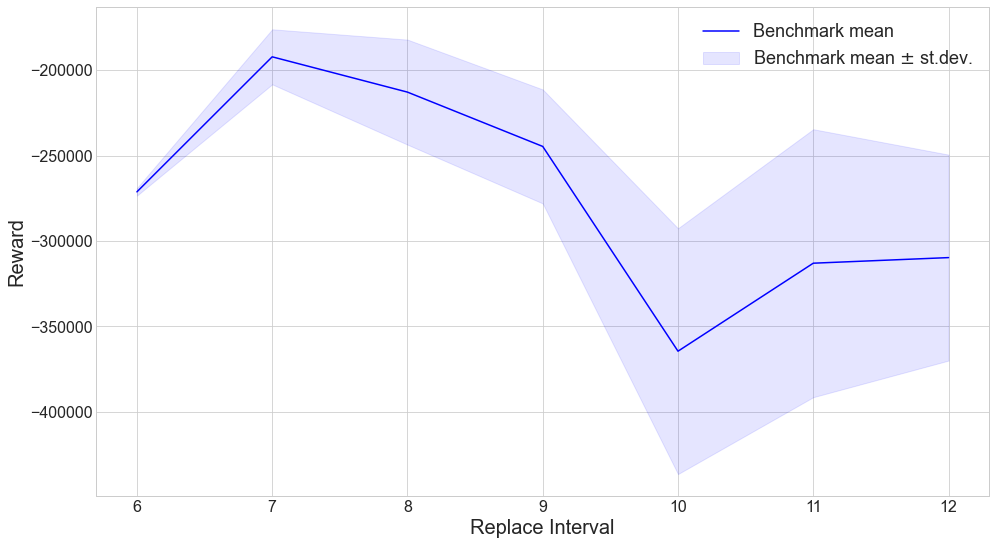
\includegraphics[width=0.8\textwidth]{Figures/tbmReplaceIntervals.png}
	\caption{\acrshort{TBM} benchmark costs over replace intervals}
	\label{tbmRplIntervals}
\end{figure}

It is observed that the optimal maintenance strategy in a periodic fashion, would be to perform a total replacement of all components every 7 decision steps. Furthermore, it is interesting to note that by increasing the replace interval there is a significantly higher variance in the rewards (maintenance costs). This is something expected, since for a shorter maintenance interval, the deterioration of the system does not evolve as much, leading to a total cost that consists almost explicitly of the maintenance actions' cost, rather than the risk of failure one.

\newpage

%------------------------------------------------------------------------------
%	RESULTS
%------------------------------------------------------------------------------

\subsection{Results}

Having elaborated on the individual sub-routines employed as well as the workflow of the complete framework, the proposed tool is applied to the 2D frame at hand. Before proceeding to the results and plots, the hyper-parameters that were used, are presented in Table \ref{ppoHyperCase}.

\begin{table}[H]
    \centering
    \caption{\gls{PPO} hyper-parameters - Case Study}
    \label{ppoHyperCase}
    \begin{tabular}{lc}
        \toprule
        \textbf{Hyper-parameter} & \textbf{Value} \\ \midrule
        gamma & $0.99$ \\
        clip ratio & $0.15$ \\
        lambda & $0.95$ \\
        number of inner layers & $2$ \\
        size of inner layers & $256$ \\
        policy learning rate &  $1.0\mathrm{E}-3$ to $2.0\mathrm{E}-5$\\
        value function learning rate & $5.0\mathrm{E}-3$ to $5.0\mathrm{E}-5$ \\ \bottomrule
    \end{tabular}
\end{table}


It should be mentioned that the learning rates that were used are not constant. To elaborate, at the beginning of the training higher values were used, i.e. $1.0\mathrm{E}-3$ and $5.0\mathrm{E}-3$ for the policy (actor network) and the value function (critic network) respectively, which serve for an initial exploration of the action and the solution space. Over the course of the training episodes, both the learning rates were refined, reaching $2.0\mathrm{E}-5$ and $5.0\mathrm{E}-5$, both to ensure a smoother training, and not to get stuck in sub-optimal solutions.

\newpage

In Figure \ref{ppoCaseResults} the training of the agent is plotted for over $6000$ episodes, along with the two benchmark thresholds (\gls{CBM} and \gls{TBM}).

\begin{figure}[H]
    \centering
    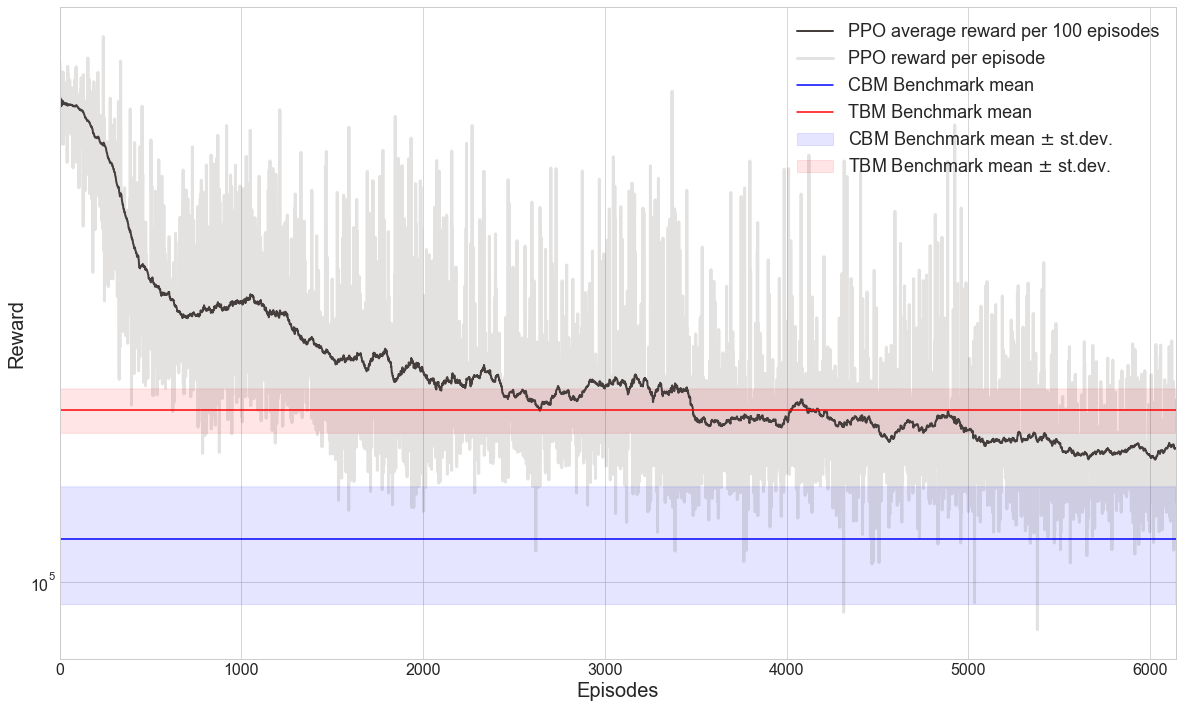
\includegraphics[width=\textwidth]{Figures/24_6100_tbm_cbm_v2.png}
	\caption{\gls{PPO} applied on case study}
	\label{ppoCaseResults}
\end{figure}

It is apparent that the proposed framework could not manage to beat both benchmarks, specifically it surpassed \gls{TBM} but not \gls{CBM}. Most probably this is the case because of the dominance of the action costs, and the small contribution of the risk of failure one. As a reminder, the total cost per decision step is decomposed as follows:

$$ R_t = C_t = C_{a_t} + C_{\text{risk}}$$

Additionally, it has been observed that the deterioration, as defined in this case study, is developing suddenly and rapidly. If there was a more gradual degradation, this would result in a probability of failure cost that would contribute significantly and during many decision steps to the total maintenance expenses. Undoubtedly, the sheer computational time needed for such a training did not allow for a proper experimentation with different hyper-parameters that would possibly perform better, reaching in the end to a better policy. Nevertheless, the agent seems to perform considerably better than the \gls{TBM} benchmark, which is not a surprise, since periodic maintenance can not account for the localization of the damage, thus, many components, that their remaining capacity is sufficient, are forced to be maintained along with the rest of the structure.\\

A way of improving the decisions of the agent, having observed that the deterioration and the resulting probability of failure, do not grow that rapidly, especially during the first decision steps, would be to include some hardcoded constraints. To be more precise, in this case, it was considered, that no maintenance action would be beneficial during the first 4 decision steps, and also no action should be made if the age (deterioration rate) of a component is less than 2. Once again many realizations were made in order to obtain a representative average maintenance cost for such a policy. The total results, both for the benchmarks and the \gls{DRL} approaches, are summarized in Table \ref{costsCase}. It should be mentioned that for all approaches, more than $100$ episodes were ran.

\begin{table}[H]
    \centering
    \caption{Benchmark and \gls{DRL} performance on the Case Study}
    \label{costsCase}
    \begin{threeparttable}
        \begin{tabular}{cccc}
            \toprule
            \textbf{\begin{tabular}[c]{@{}c@{}}Maintenance\\ Approach\end{tabular}} & \textbf{\begin{tabular}[c]{@{}c@{}}Mean\\ Cost\end{tabular}} & \textbf{\begin{tabular}[c]{@{}c@{}}St. Dev.\\ Cost\end{tabular}} & \textbf{\begin{tabular}[c]{@{}c@{}}Relative\\ Difference\tnote{*}\end{tabular}} \\ \midrule
            \acrshort{CBM} Benchmark & 117820.0 & 25854.9 & 100.00\% \\
            \acrshort{TBM} Benchmark & 192069.2 & 16121.0 & 163.02\% \\
            \gls{PPO} & 166148.2 & 27809.7 & 141.02\% \\
            Constrained \gls{PPO} & 133368.7 & 11180.2 & 113.20\%\\
            \bottomrule
        \end{tabular}
        \begin{tablenotes}
            \item[*] \footnotesize{The mean cost achieved by each approach is compared with the minimum of all, i.e. the \acrshort{CBM} Benchmark one}
        \end{tablenotes}
    \end{threeparttable}
\end{table}

The fact that a constrained \gls{PPO} agent can arrive at lower maintenance costs, proves that a better tuning of the hyper-parameters can yield more efficient policies. \\

What is more, another interesting plot is the policy realization for the constrained agent. Of course, a single realization is not the most representative, but it still provides a qualitative representation of how the agent chooses its actions. Such a plot, is displayed in Figure \ref{2DframePolReal}, where the damage over the time horizon and the corresponding actions are plotted for all the components.


\begin{figure}[H]
    \centering
    \makebox[\textwidth][c]{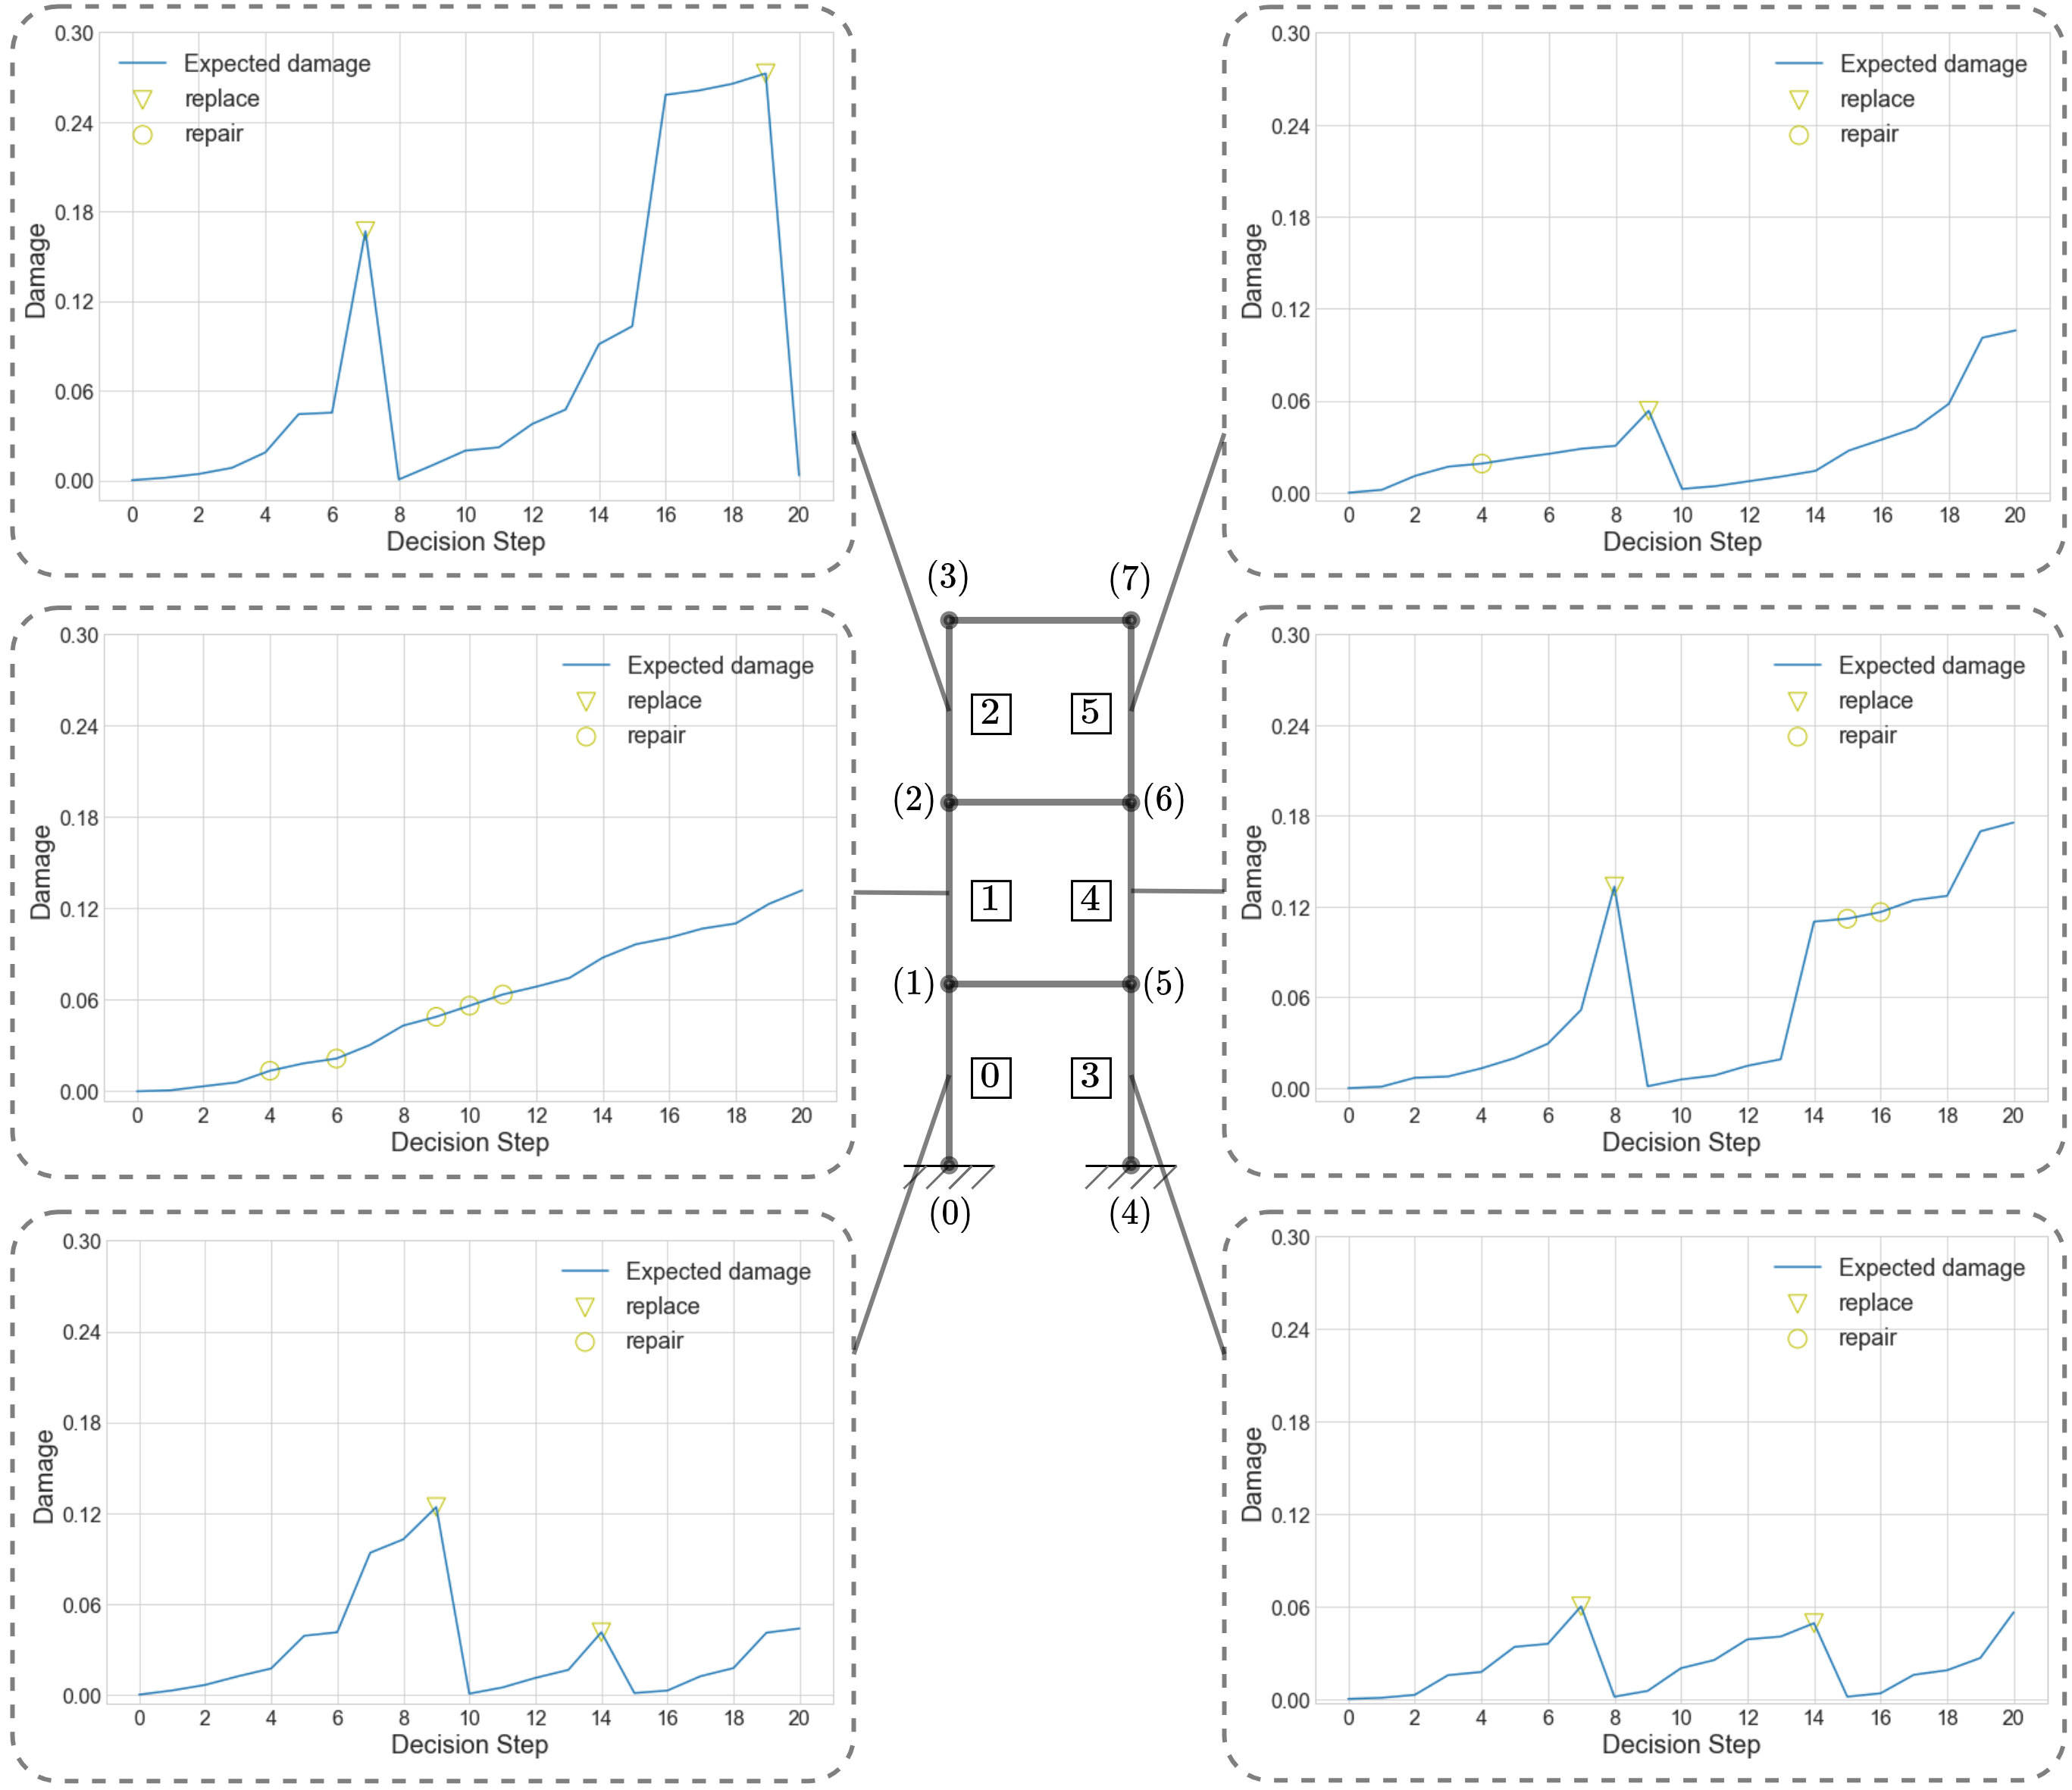
\includegraphics[width=1.2\textwidth]{Figures/fullFramePolReal.png}}
	\caption{Policy realization for all components (constrained)}
	\label{2DframePolReal}
\end{figure}

\newpage

It is evident that there is not a specific pattern that the agent follows neither on a global scale nor on a component one. Undoubtedly, it does not allow the damage to reach extremely high values, since this would also affect significantly the horizontal displacement of the top storey, which is the control quantity for the structure's failure. \\

In Figures \ref{3dPolEpsL} and \ref{3dPolEpsR}, policy realizations are plotted for different levels of training. In particular, there is a policy realization every $1200$ episodes, to demonstrate the learning of the agent, and how from completely uninformed and random actions, it shifted to more reasonable and beneficial ones. To serve this purpose from a presentation point of view, a color-bar is included in the plots, to display the decrease of the total maintenance costs over the course of training episodes.

\begin{figure}[H]
    \centering
    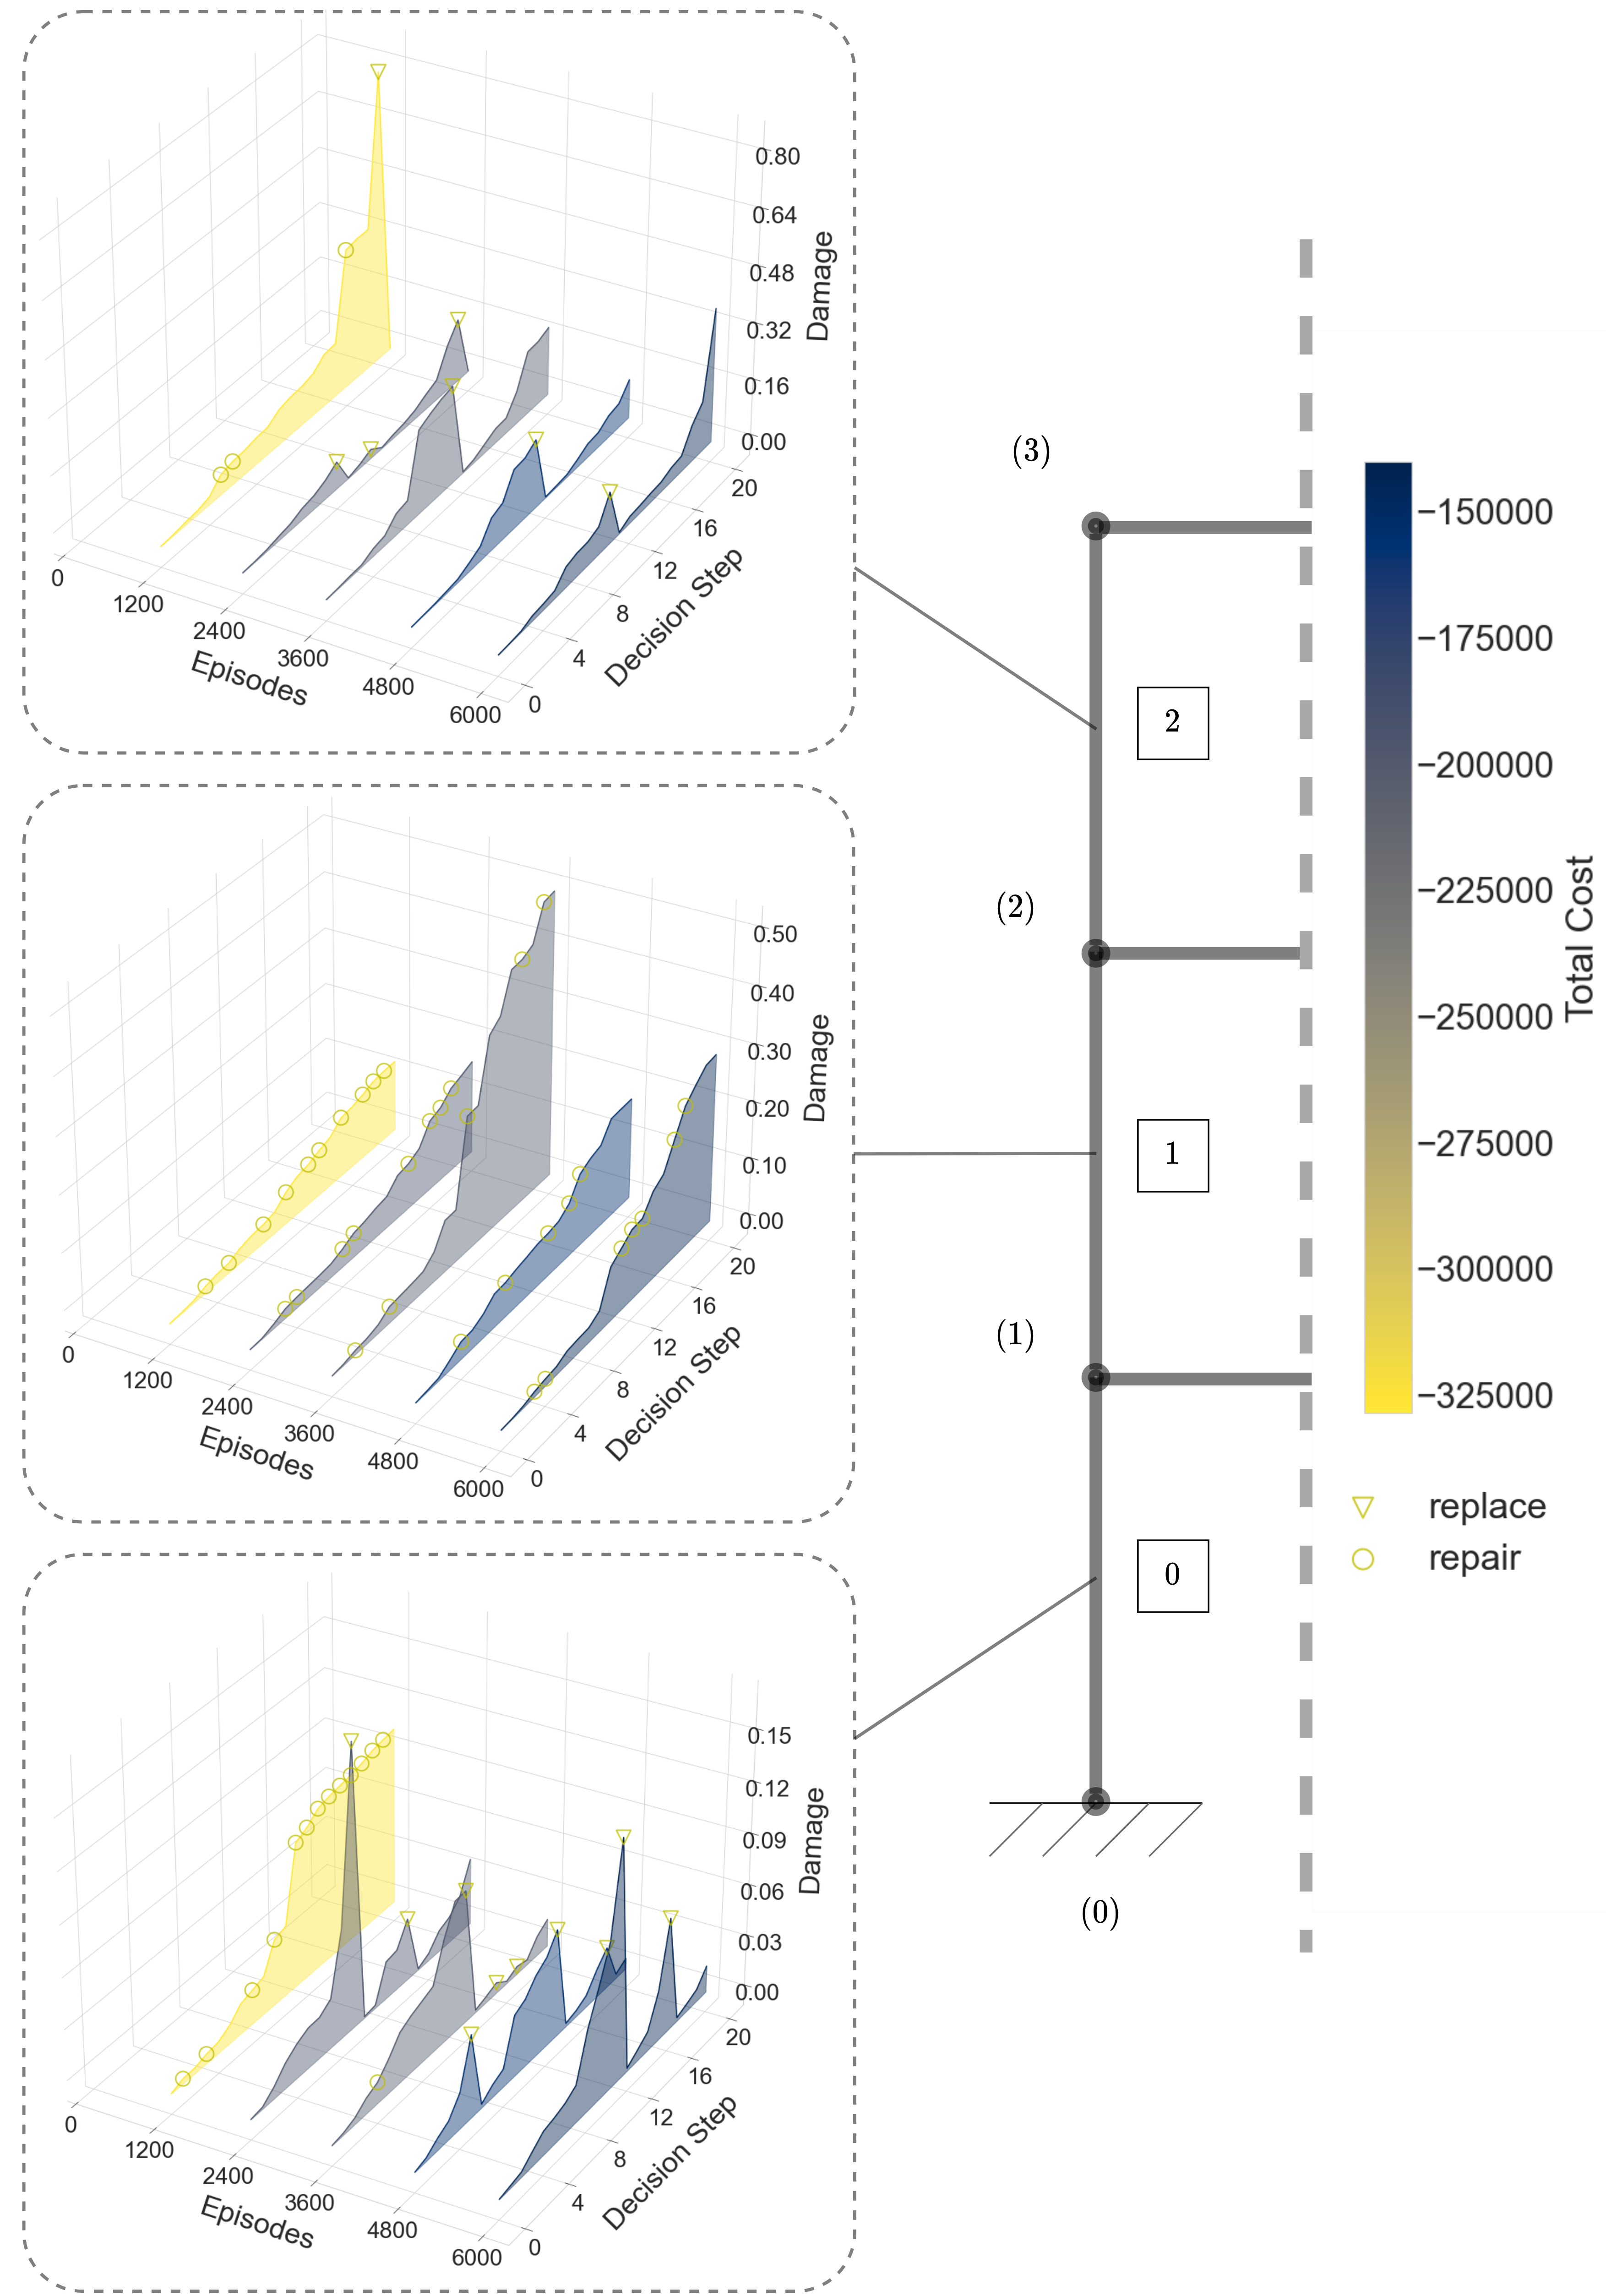
\includegraphics[width=.95\textwidth]{Figures/leftFrame.png}
	\caption{Policy realization for all components for different training episodes - Left side}
	\label{3dPolEpsL}
\end{figure}

\begin{figure}[H]
    \centering
    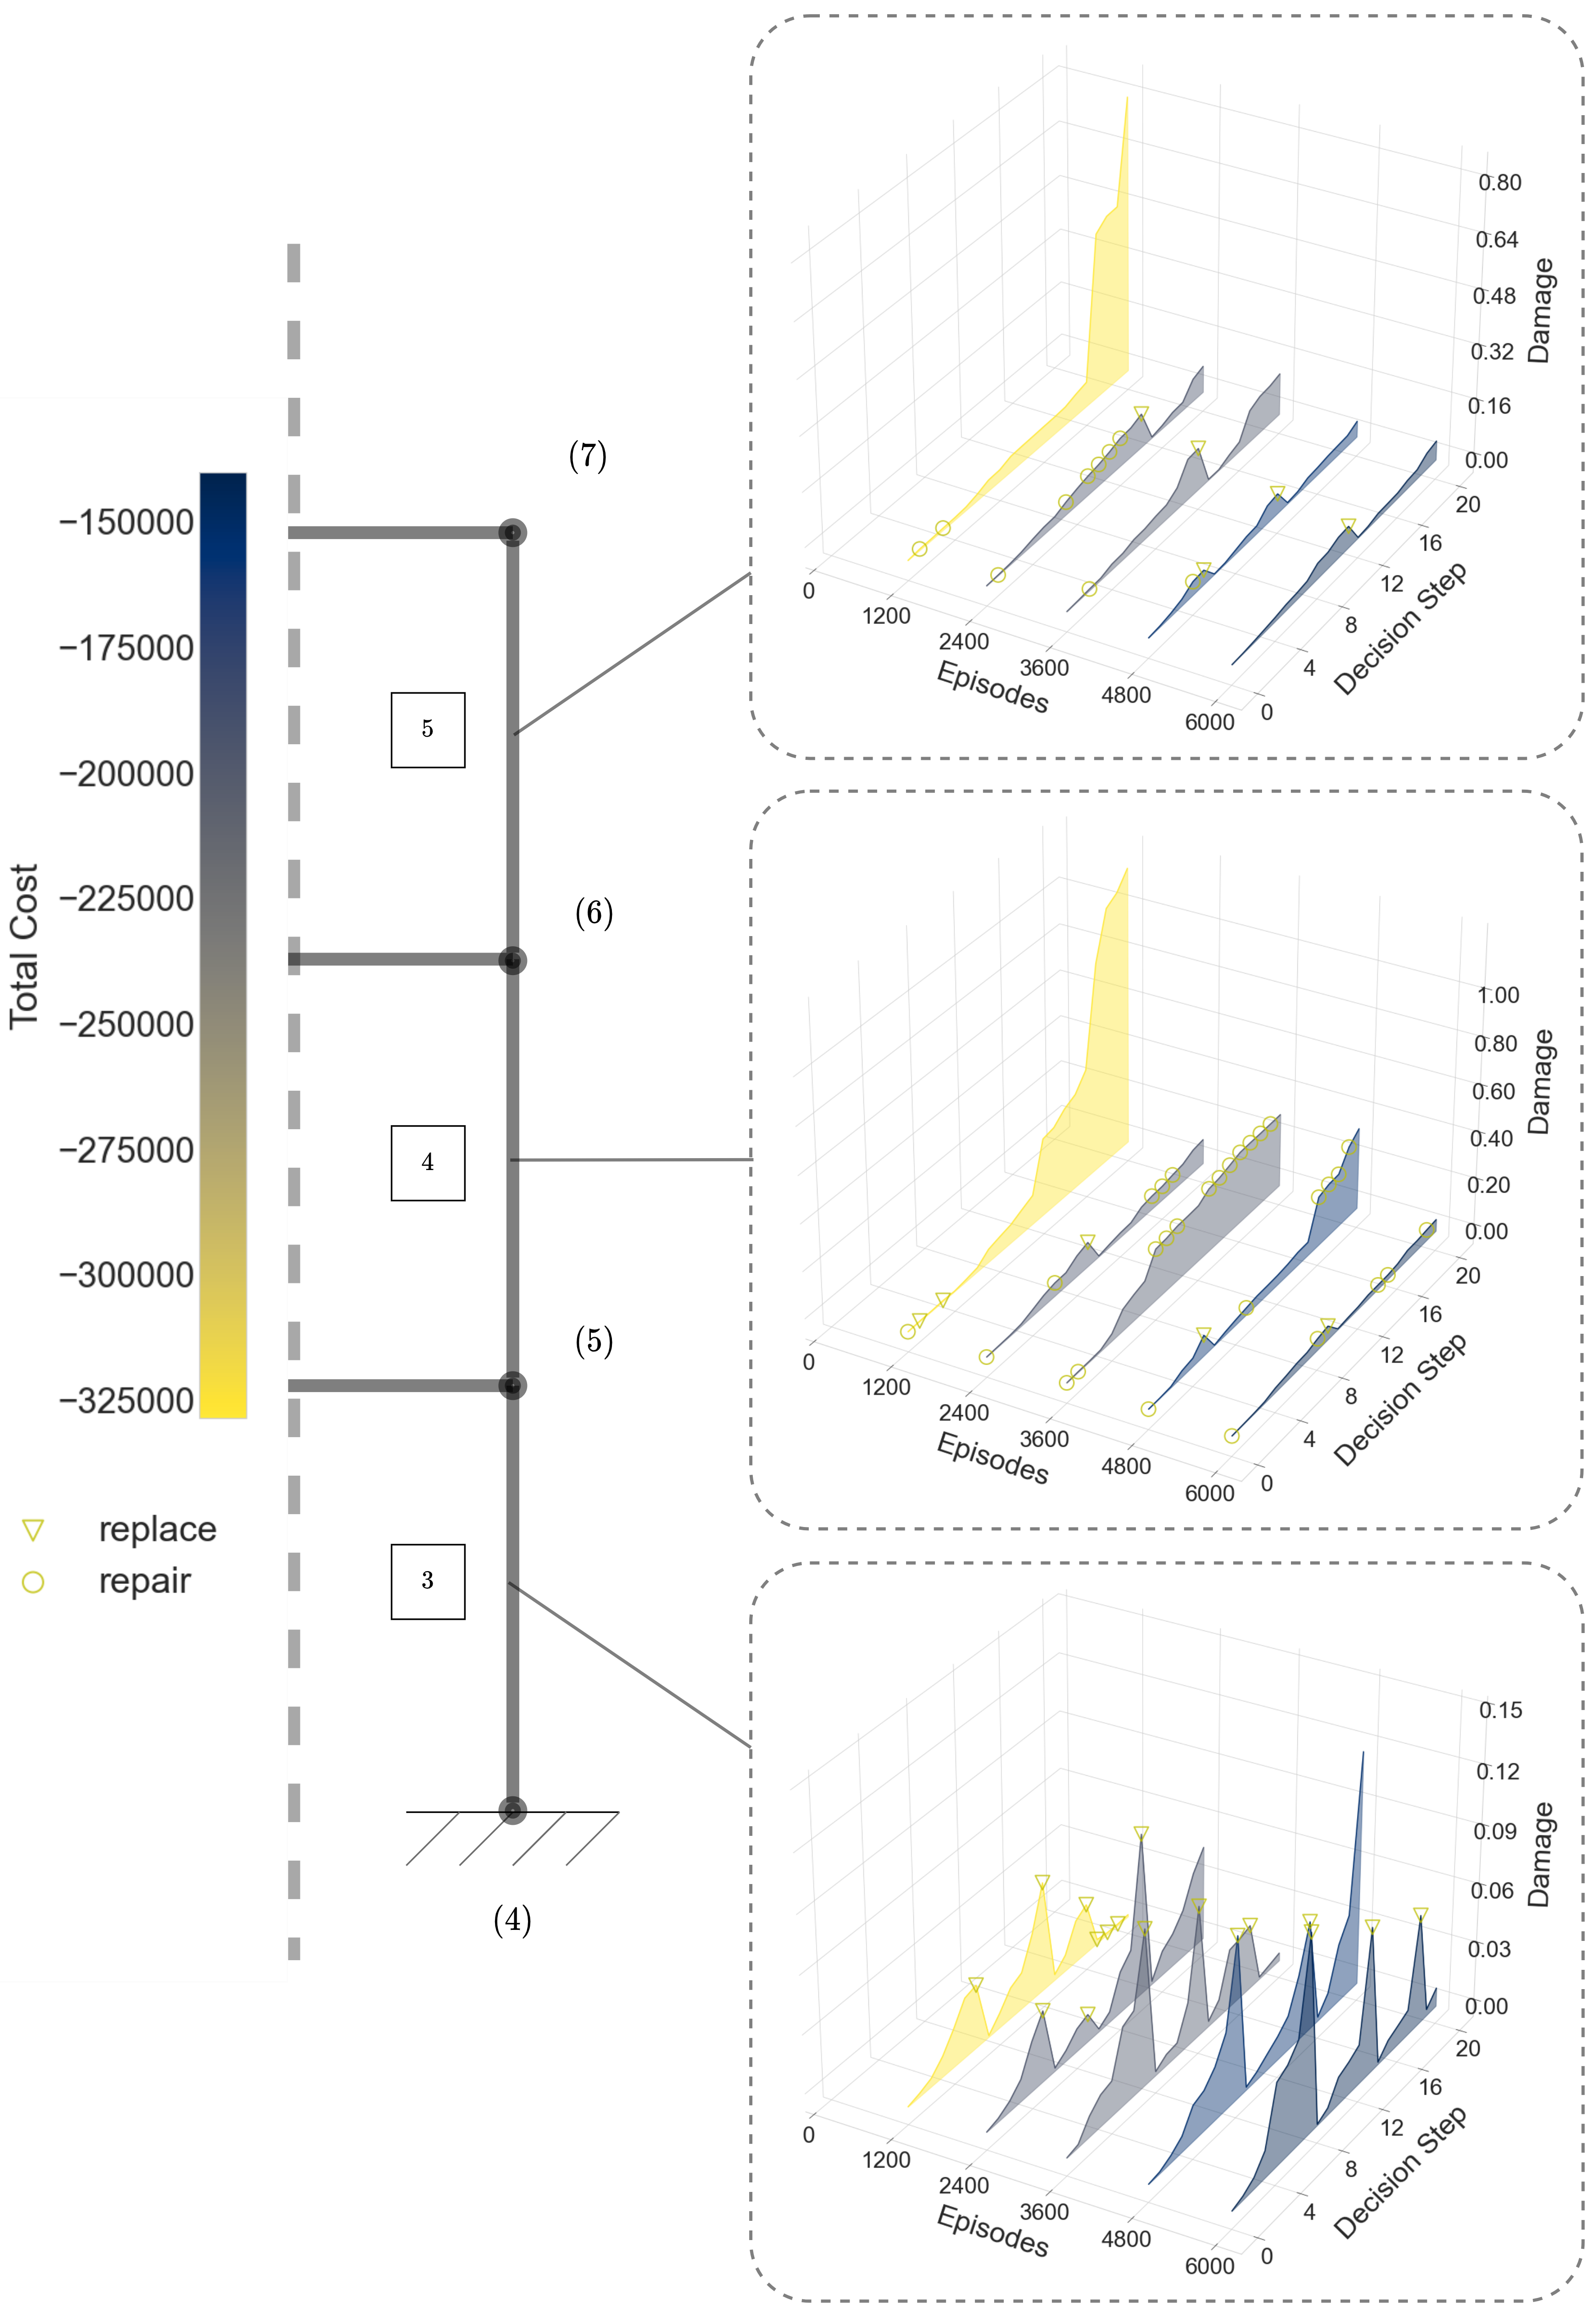
\includegraphics[width=.95\textwidth]{Figures/rightFrame.png}
	\caption{Policy realization for all components for different training episodes - Right side}
	\label{3dPolEpsR}
\end{figure}

It goes without saying, that the agent during the early learning stages was allowing the deterioration to grow significantly, something that changed over the course of more episodes, since higher damage values combined with the degradation of other components as well can lead to a greater probability of failure $P_f$. Another interesting observation is that, especially for the left side of the frame, the agent gets much more sensitive about the damage of the base storey, rather than the ones of the two above. This is a reasonable strategy, because the damage of the lowest column has a greater contribution to the global failure. Surprisingly, this is not the same case for the right side, where all columns are limited to small damage values, regardless from their location. As already explained, this could be attributed to the high stochasticity of the corrosive environment, which makes a single realization a non-representative measure.

%------------------------------------------------------------------------------
%	CONCLUSIONS
%------------------------------------------------------------------------------

\subsection{Conclusions}

Summarizing the chapter, some general comments will be made and conclusions will be drawn, regarding the case study.\\

Moving from a simplistic application such as the toy problem, to a more complicated case study undoubtedly made the optimal maintenance strategy harder to determine. The considered 2D frame is a multi-component system that poses greater challenges, with the more obvious one being the enhancement of the action and state spaces. The benchmark approach, and more specifically the \gls{CBM} version of it, was more difficult to beat, and it was highlighted that a better tuning of the hyper-parameters is necessary. It is also possible that the initial problem setup needs to be reconsidered, and particularly the assumptions made about the costs/rewards during every decision~step.